\clearpage
\section{الخدمات}
\label{sec:builder-feature-services}

الخدمة هي ما يظهر للمتعاملين على بوابة المؤسسة، مثل «طلب شهادة» أو «حجز موعد». وتضم كل خدمة نموذجاً أو أكثر، وتحدد طريقة تقديمها ومن يحق له التقديم. لذلك لا يصل النموذج إلى المتعاملين إلا عبر خدمة، أما النموذج الذي لا ينتمي إلى خدمة فيبقى نموذجاً داخلياً يستخدمه الموظفون فقط. وتجمع صفحة «الخدمات» الخدمات كلها في جدول واحد، ومنها تنشئ خدمة جديدة وتفتح مكتب الاستقبال وأداء الخدمات.

\textbf{المسار ومن يستخدمه:} «ادوات البناء» ← «الأساسية» ← «الخدمات». يستخدمها من يدير الخدمات العامة للمؤسسة، عند إنشاء خدمة أو مراجعة حالة الخدمات القائمة.

\begin{rcnote}[مثال: شركة الأفق]
يضغط مسؤول النظام في الأفق «خدمة جديدة» ①، ويسمّي الخدمة «طلب زيارة فرع»، ويختار «هجينة» لأن الطلب يبدأ عبر البوابة وتجري الزيارة نفسها في فرع حلب. ثم يختار النموذج المنشور «طلب زيارة فرع»، بينما تبقى نماذج الأفق الأخرى في «نماذج داخلية» ④.
\end{rcnote}

\begin{figure}[H]
\centering
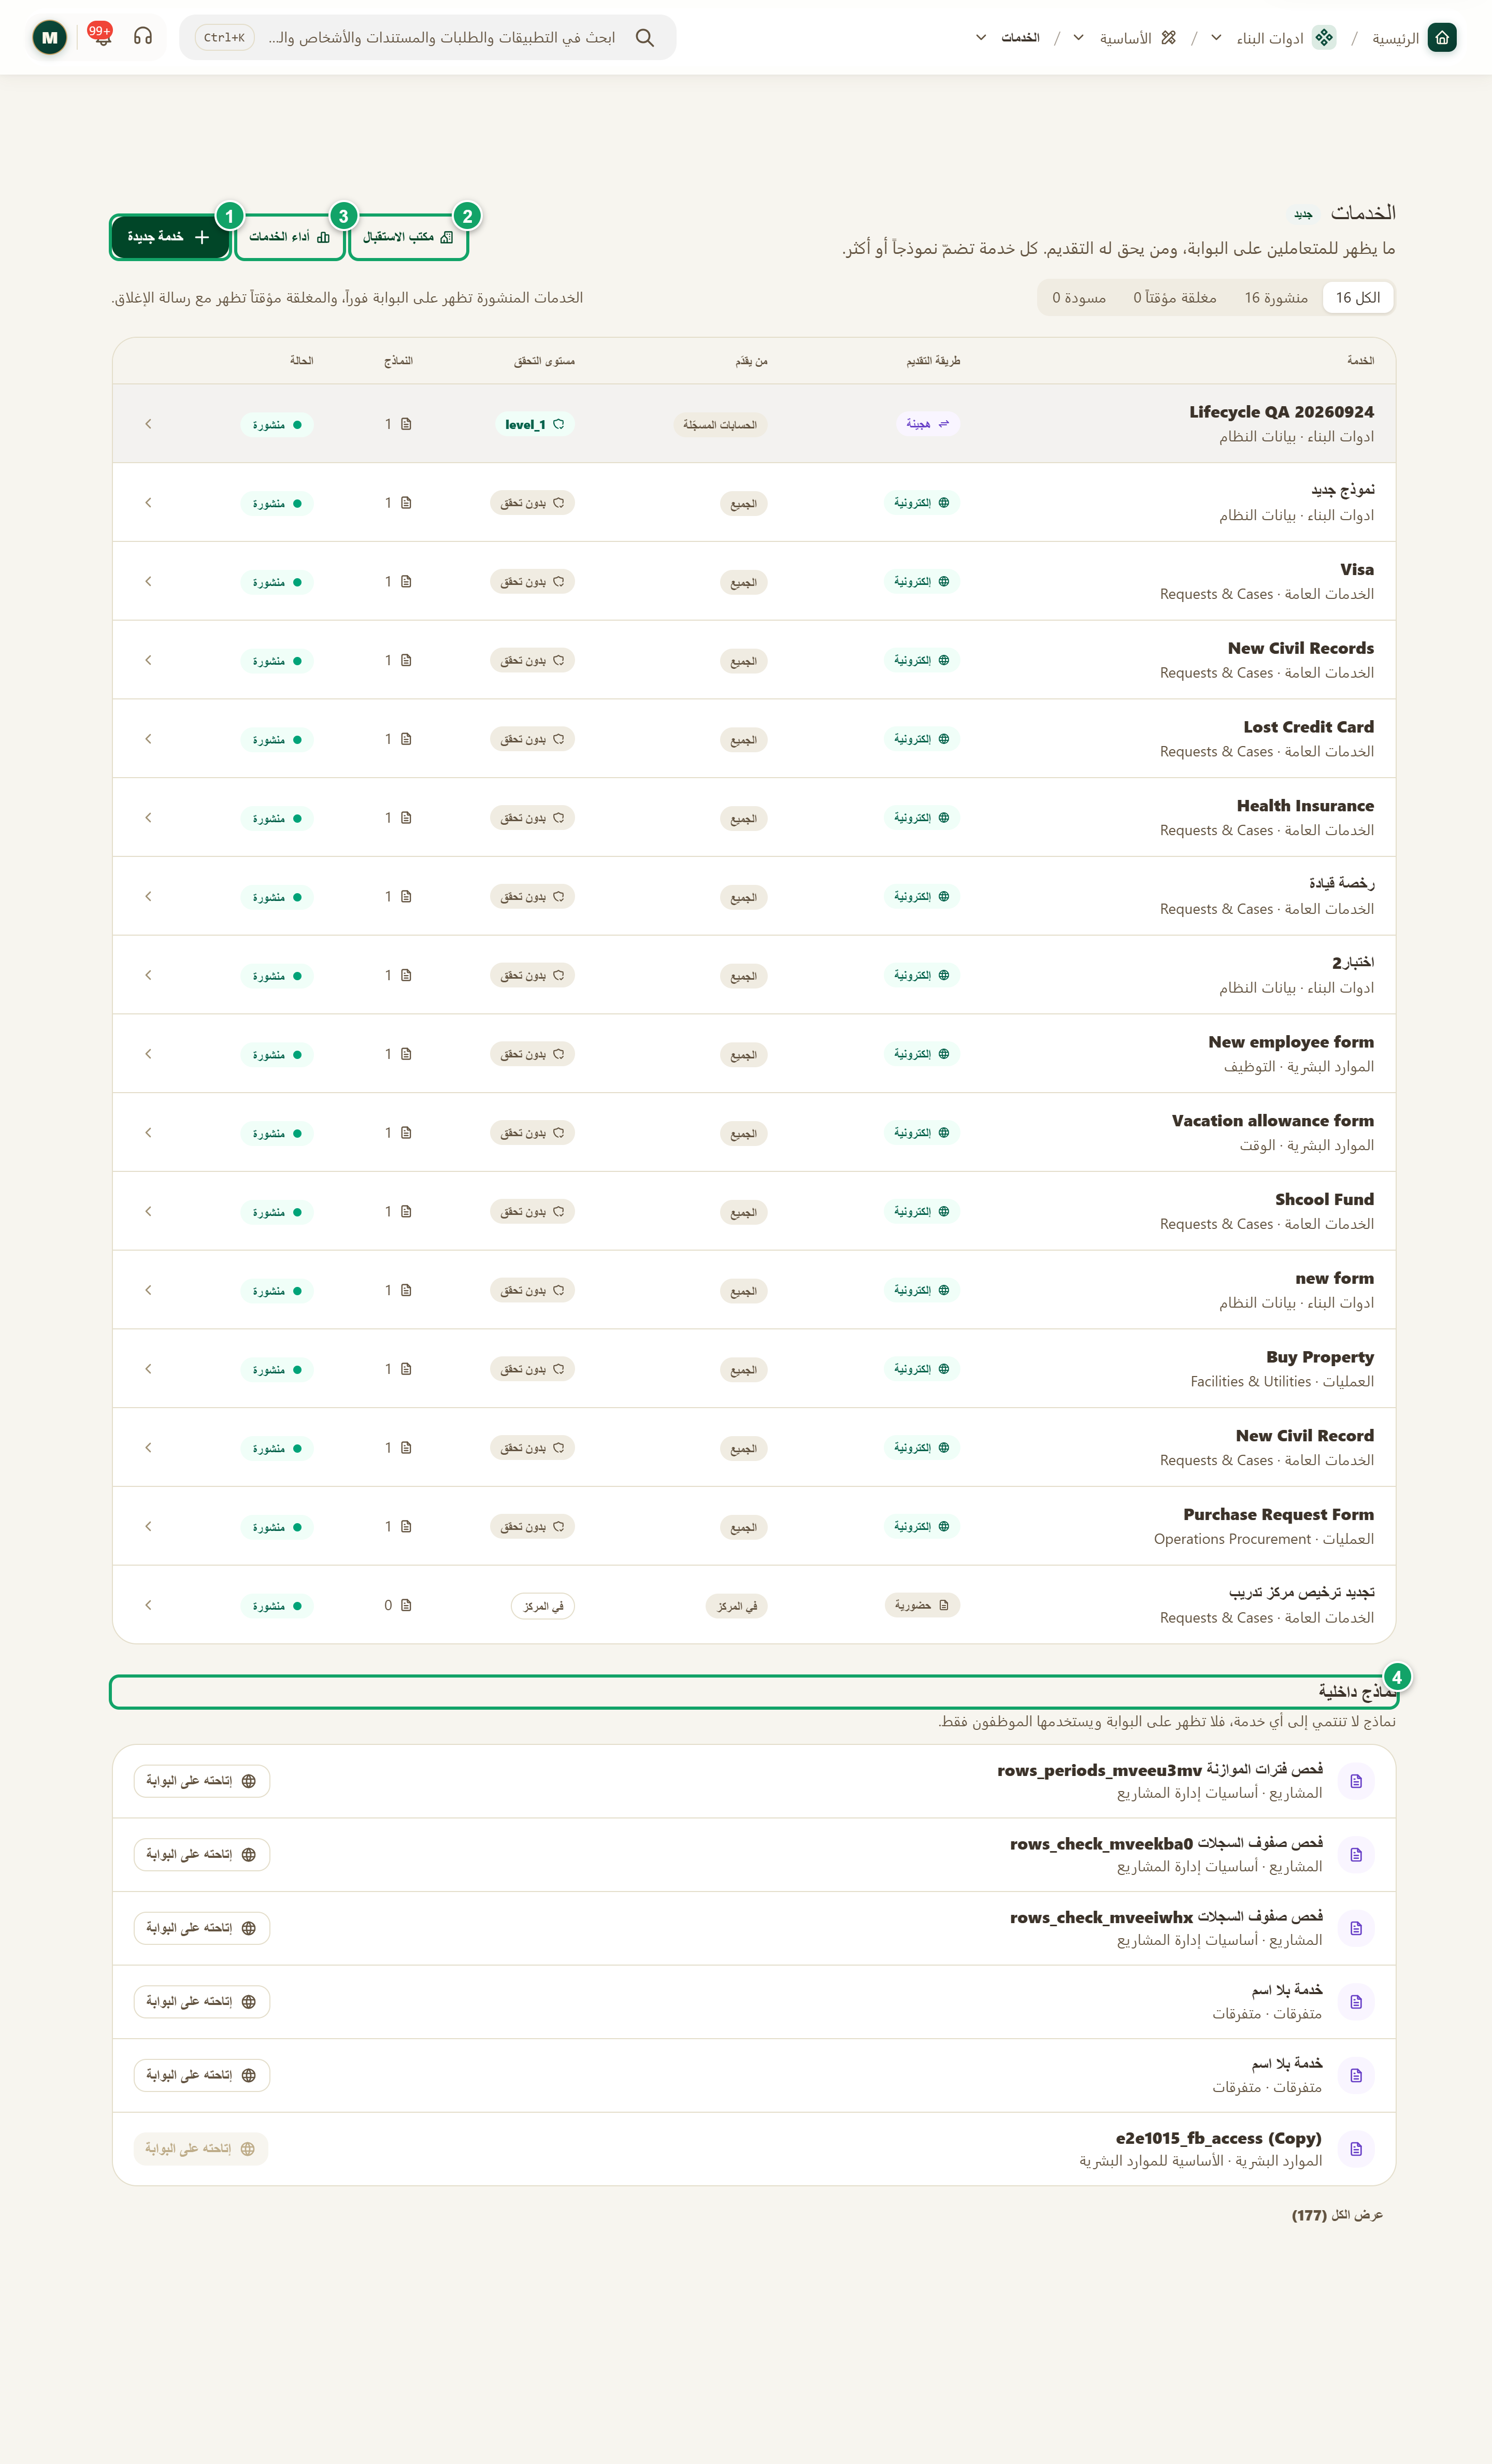
\includegraphics[width=0.95\linewidth,height=0.72\textheight,keepaspectratio]{figures/screens/ch06-services-ar.png}
\caption{صفحة «الخدمات»}
\label{fig:builder-services-screen}
\shotnote{تعرض الصفحة الخدمات التي تظهر على البوابة وحالتها، ثم النماذج الداخلية التي لا تنتمي إلى خدمة. ① «خدمة جديدة»: تبدأ خدمة حول نموذج منشور. ② «مكتب الاستقبال»: يسجّل طلباً حضورياً. ③ «أداء الخدمات». ④ «نماذج داخلية»: النماذج التي لا يراها الجمهور.}
\end{figure}

\begin{figure}[H]
\centering
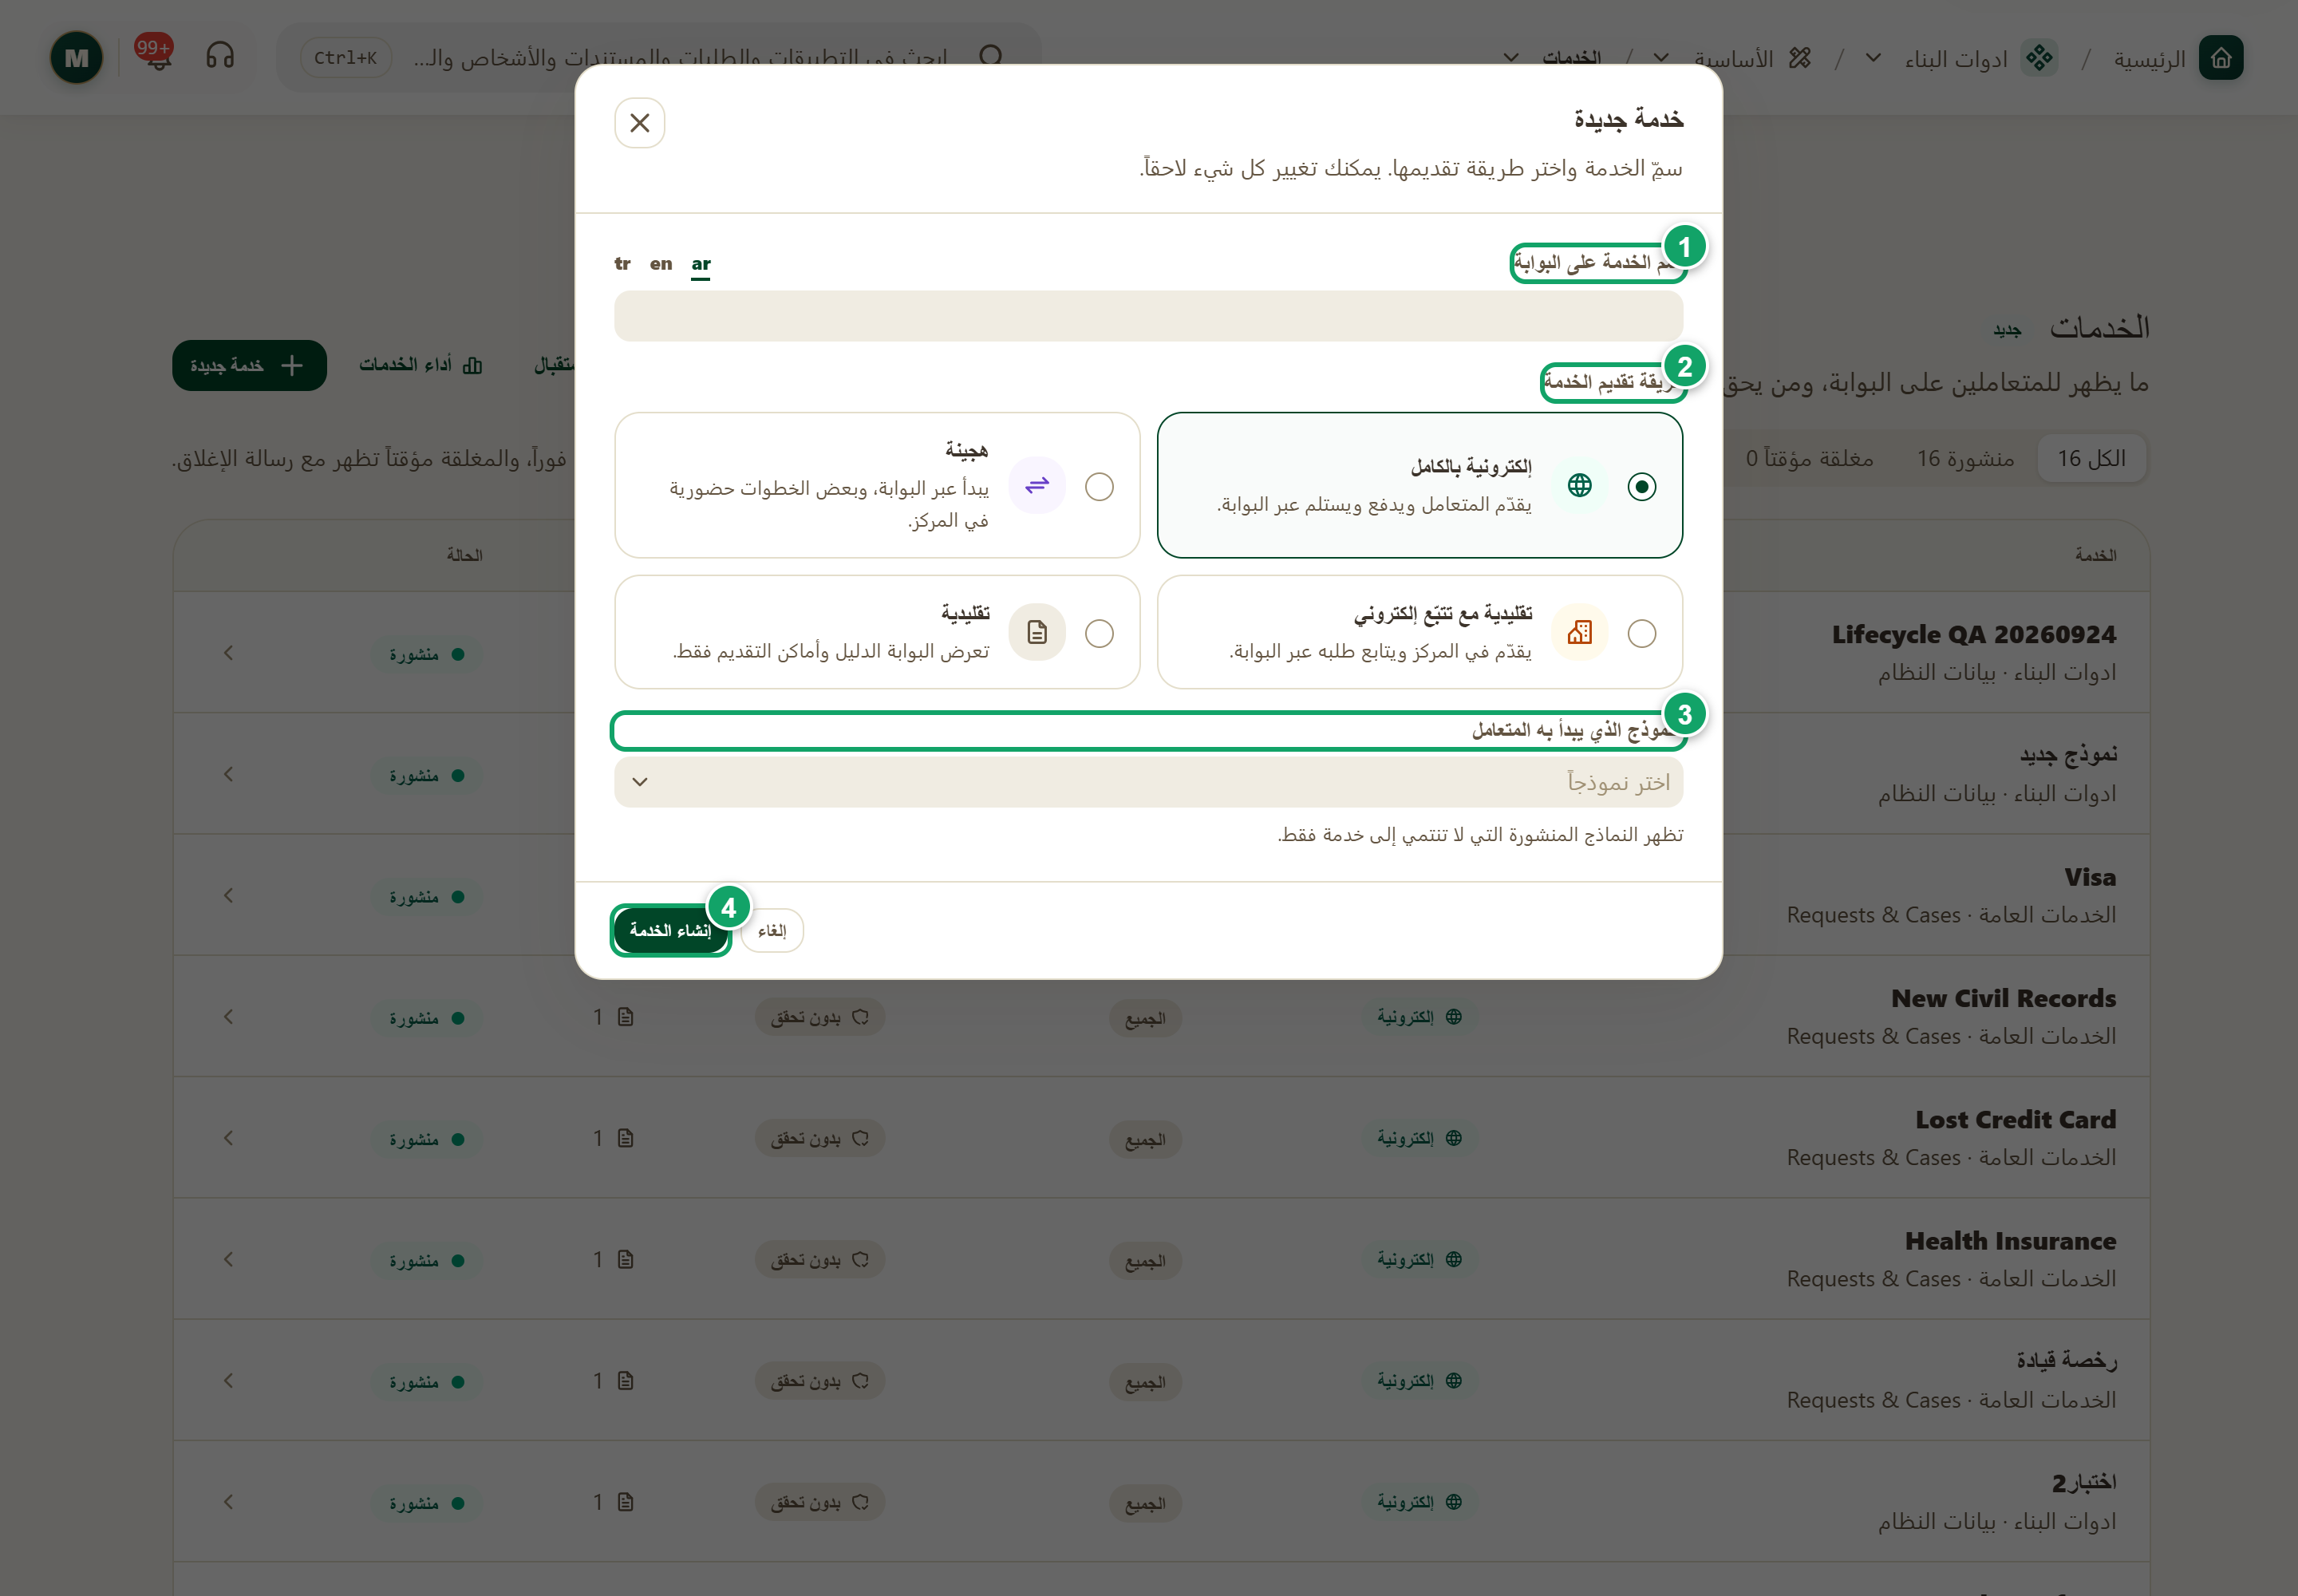
\includegraphics[width=0.95\linewidth,height=0.72\textheight,keepaspectratio]{figures/screens/ch06-services-new-ar.png}
\caption{نافذة «خدمة جديدة»}
\label{fig:builder-services-new-screen}
\shotnote{تعرض الصورة نافذة «خدمة جديدة» قبل تعبئتها في مؤسسة الاختبار، وفيها الطرق الأربع لتقديم الخدمة. وتبيّن أن إنشاء الخدمة لا يطلب سوى ثلاثة أشياء، أما بقية الإعدادات فتُستكمل لاحقاً من صفحة الخدمة. ① «اسم الخدمة على البوابة». ② «طريقة تقديم الخدمة»: تحدد هل تبدأ الخدمة عبر البوابة أو في المركز. ③ «النموذج الذي يبدأ به المتعامل»: لا تعرض القائمة إلا النماذج المنشورة التي لا تنتمي إلى خدمة. ④ «إنشاء الخدمة»: ينشئ الخدمة مسودةً ويفتح صفحتها.}
\end{figure}

\begin{table}[H]
\centering
\caption{ما الذي تجده في صفحة «الخدمات»؟}
\label{tab:builder-services-data}
\begin{tabularx}{\linewidth}{R{3.6cm} Y}
\rcHeaderRow
\thh{الجزء} & \thh{المحتوى والإجراء}\\
جدول الخدمات & يعرض لكل خدمة «طريقة التقديم» و«من يقدّم» و«مستوى التحقق» وعدد «النماذج» و«الحالة»، والضغط على الصف يفتح صفحة الخدمة.\\
تصفية حسب الحالة & تعرض «الكل» أو «منشورة» أو «مغلقة مؤقتاً» أو «مسودة» مع عدد كل منها. والمنشورة تظهر على البوابة فوراً، والمغلقة مؤقتاً تظهر مع رسالة الإغلاق.\\
من إعدادات النموذج & شارة لنموذج منشور للعامة بإعداداته القديمة دون خدمة، وزر «إنشاء خدمة» يحوّله إلى خدمة تديرها من هنا.\\
نماذج داخلية & نماذج لا تنتمي إلى أي خدمة، ولكل منها زر «إتاحته على البوابة» الذي يعمل بعد نشر النموذج.\\
خدمة جديدة & نافذة تطلب «اسم الخدمة على البوابة» و«طريقة تقديم الخدمة» والنموذج الذي تبدأ به الخدمة، ثم تُنشأ الخدمة مسودةً وتفتح صفحتها.\\
\end{tabularx}
\end{table}

\begin{table}[H]
\centering
\caption{طرق تقديم الخدمة}
\label{tab:builder-services-modes}
\begin{tabularx}{\linewidth}{R{3.6cm} Y}
\rcHeaderRow
\thh{الطريقة} & \thh{ما تعنيه وما تطلبه عند الإنشاء}\\
إلكترونية بالكامل & يقدّم المتعامل ويدفع ويستلم عبر البوابة، وكل خطوات المسار نماذج. وتطلب «النموذج الذي يبدأ به المتعامل»، ولا تظهر في القائمة إلا النماذج المنشورة التي لا تنتمي إلى خدمة.\\
هجينة & يبدأ الطلب عبر البوابة، وتجري بعض الخطوات حضورياً في مركز الخدمة. وتطلب نموذج البدء نفسه.\\
تقليدية مع تتبّع إلكتروني & يُقدَّم الطلب في المركز ويتابعه المتعامل على البوابة برقم الطلب ورقم الهاتف. ويمكنك أن تختار «نموذج يعبّئه الموظف (اختياري)».\\
تقليدية & لا طلبات على البوابة، بل تعرض الدليل وأماكن التقديم فقط، ويمكن للموظفين تسجيل الطلب داخلياً. والنموذج هنا اختياري أيضاً.\\
\end{tabularx}
\end{table}

\begin{figure}[H]
\centering
\begin{tikzpicture}[node distance=0.5cm]
\node[entity] (service) {\RL{الخدمة}};
\node[entity,below right=0.7cm and 0.3cm of service] (entry) {\RL{نموذج البداية}};
\node[entityOpt,below left=0.7cm and 0.3cm of service] (more) {\RL{نماذج المسار والمتابعة}};
\draw[dependsOn] (service.south) -- ++(0,-0.3) -| (entry.north);
\draw[dependsOnOpt] (service.south) -- ++(0,-0.3) -| (more.north);
\end{tikzpicture}
\rclegend
\caption{ما تضمه الخدمة}
\label{fig:builder-services-model}
\shotnote{يوضّح الشكل أن الخدمة التي تبدأ عبر البوابة تحتاج إلى نموذج بداية منشور يعبّئه المتعامل، وأن بقية النماذج اختيارية، مثل خطوات لاحقة في المسار أو نموذج متابعة يُطلب عند حالة معينة. لذلك انشر النموذج في منشئ النماذج أولاً، ثم أنشئ الخدمة حوله.}
\end{figure}

\subsection{خطوات العمل والتحقق}
\begin{enumerate}
\item انشر النموذج الذي سيبدأ به المتعامل من صفحة «النماذج».
\item افتح «الخدمات» واضغط «خدمة جديدة»، واكتب «اسم الخدمة على البوابة».
\item اختر «طريقة تقديم الخدمة»، ثم اختر النموذج من القائمة واضغط «إنشاء الخدمة».
\item أكمل تبويبات صفحة الخدمة: «التعريف» و«التقديم والأهلية» و«المسار والنماذج» و«الرسوم».
\item غيّر «حالة الخدمة» إلى «منشورة»، ثم اضغط «عرض على البوابة» لتراها كما يراها المتعامل.
\end{enumerate}

\textbf{تحقق ومعالجة المشكلة:} تظهر الخدمة الجديدة في الجدول بحالة «مسودة»، ولا تظهر على البوابة حتى تنشرها، لأن «المسودة لا تظهر على البوابة». وإذا لم تجد نموذجك في قائمة الإنشاء، فتأكد من أنه منشور ولا ينتمي إلى خدمة أخرى. وإذا أردت إيقاف الطلبات مؤقتاً، فاجعل الخدمة «مغلقة مؤقتاً» مع رسالة للمتعاملين بدلاً من حذفها.

\clearpage
\section{نظرة عامة على الخدمة}
\label{sec:builder-feature-services-overview}

تفتح كل خدمة على تبويب «نظرة عامة»، وهو ملخص يجيب عن ثلاثة أسئلة: هل الخدمة جاهزة، وكيف يسير أداؤها، وما الذي يحتاج إلى تدخلك الآن. وتبدأ الصفحة بقائمة «جاهزية الخدمة» التي تفحص كل جزء من إعدادها، ثم أرقام آخر 30 يوماً، ثم الطلبات المتأخرة. لذلك عُد إليها كلما فتحت الخدمة لتعرف أين تبدأ.

\textbf{المسار ومن يستخدمه:} «الخدمات» ← اضغط الخدمة ← «نظرة عامة». يستخدمها من يبني الخدمة ليكمل إعدادها، ومن يتابعها ليرى ما تأخر من طلباتها.

\begin{rcnote}[مثال: شركة الأفق]
يفتح مسؤول النظام خدمة «طلب زيارة فرع» فيجد في «جاهزية الخدمة» ① أن «الرسوم» غير معدّة وأن «الاستقبال في المركز» متوقف. فيضغط «تفعيل» بجانب الاستقبال لينتقل مباشرة إلى تبويب «التقديم والأهلية».
\end{rcnote}

\begin{figure}[H]
\centering
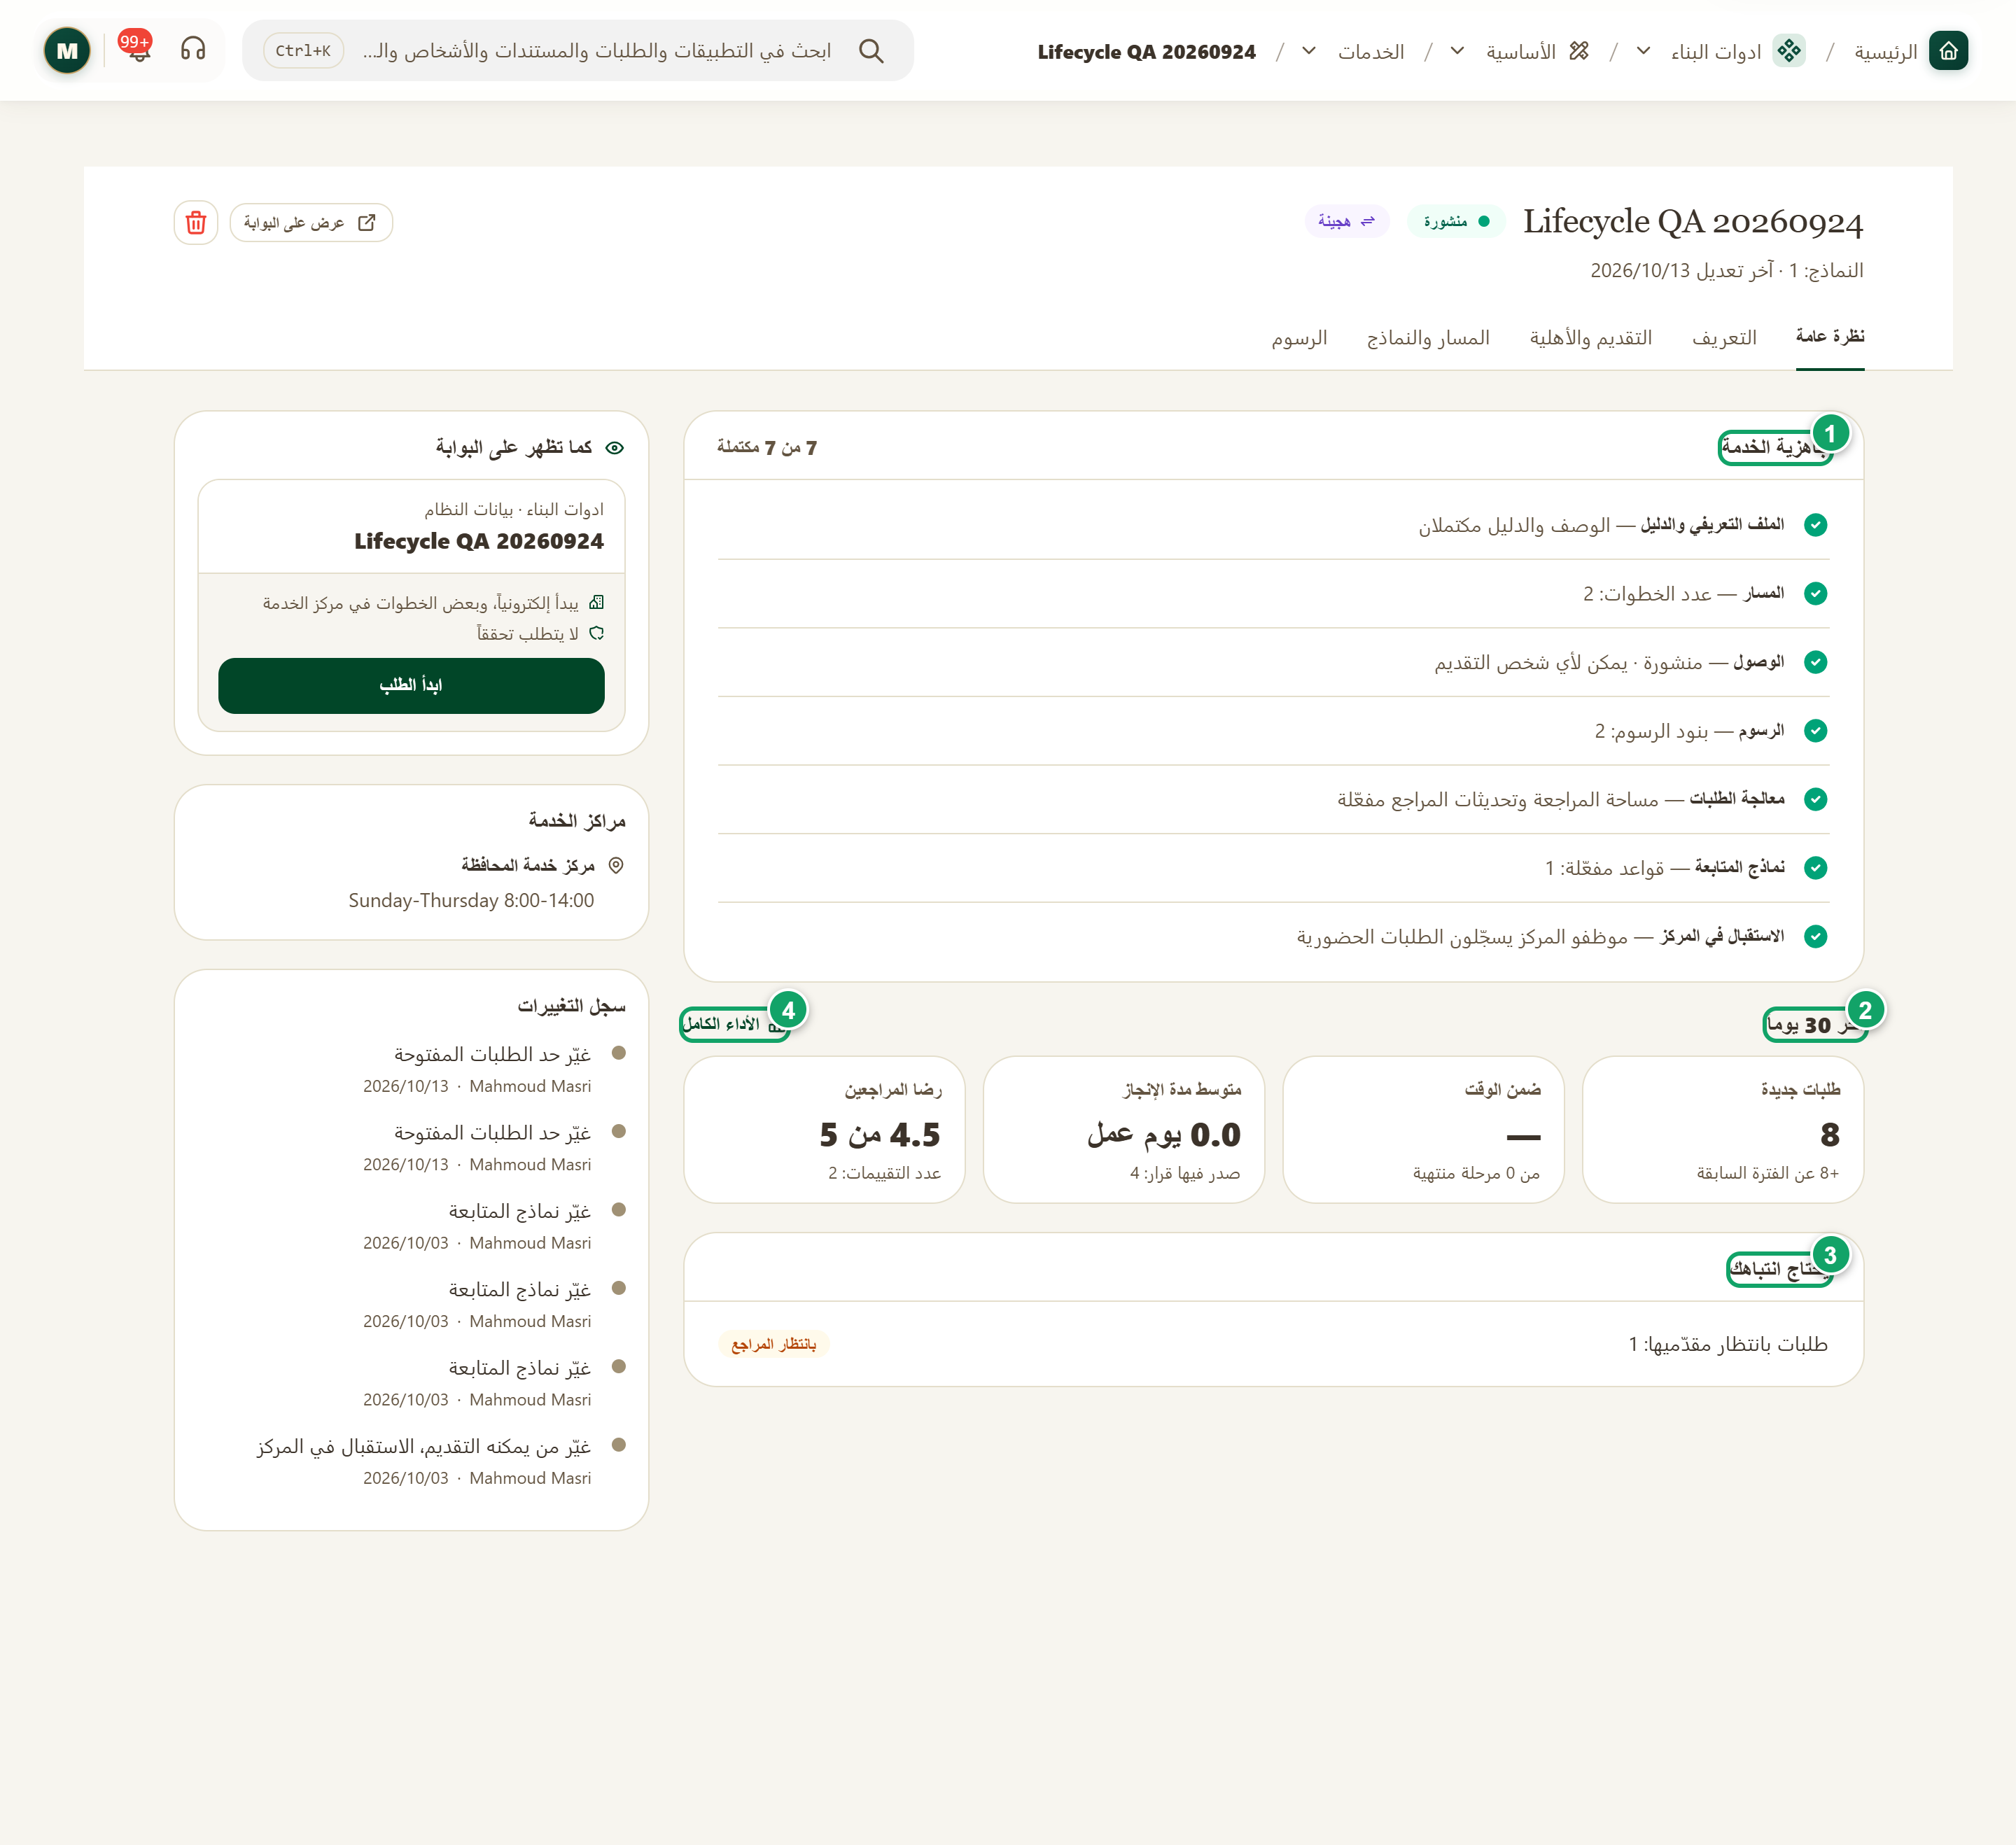
\includegraphics[width=0.95\linewidth,height=0.72\textheight,keepaspectratio]{figures/screens/ch06-services-overview-ar.png}
\caption{تبويب «نظرة عامة» لخدمة في مؤسسة الاختبار}
\label{fig:builder-services-overview-screen}
\shotnote{تعرض الصورة خدمة هجينة منشورة في مؤسسة الاختبار اكتملت بنود جاهزيتها السبعة، ومعها أرقام آخر 30 يوماً وطلب واحد ينتظر مقدّمه. وتبيّن أن هذا التبويب يجمع حالة الإعداد وحالة الطلبات في شاشة واحدة، فتعرف منه ما يحتاج إلى إكمال وما يحتاج إلى متابعة. ① «جاهزية الخدمة»: البنود التي تفحص إعداد الخدمة مع عدّاد المكتمل منها. ② «آخر 30 يوماً». ③ «يحتاج انتباهك»: الطلبات المتأخرة أو التي تنتظر مقدّميها. ④ «الأداء الكامل»: يفتح صفحة «أداء الخدمات».}
\end{figure}

\begin{table}[H]
\centering
\caption{بنود «جاهزية الخدمة»}
\label{tab:builder-services-overview-checks}
\begin{tabularx}{\linewidth}{R{3.6cm} Y}
\rcHeaderRow
\thh{البند} & \thh{متى يكتمل}\\
الملف التعريفي والدليل & عندما يكون للخدمة وصف، ومعه مدة الإنجاز أو مستند مطلوب واحد على الأقل في الدليل.\\
المسار & عندما يضم المسار خطوة واحدة على الأقل، ويظهر عدد الخطوات.\\
الوصول & عندما تكون الخدمة «منشورة»، ويذكر البند أيضاً هل تتطلب حساباً ومستوى التحقق المطلوب.\\
الرسوم & عندما تُفعَّل بنود الرسوم وفيها بند واحد على الأقل. أما إذا كُتبت الرسوم نصاً في الدليل فقط، فينبّهك البند إلى تحويلها إلى بنود.\\
معالجة الطلبات & عندما تُفعَّل مساحة المراجعة وتحديثات المراجع لنموذج البدء.\\
نماذج المتابعة & عندما تُفعَّل نماذج المتابعة، ويظهر عدد القواعد المفعّلة.\\
الاستقبال في المركز & يظهر للخدمات التي فيها خطوات حضورية فقط، ويكتمل عندما يسجّل موظفو المركز الطلبات الحضورية.\\
\end{tabularx}
\end{table}

وبجانب كل بند غير مكتمل رابط ينقلك إلى التبويب الذي يصلحه، مثل «استكمال» أو «فتح الرسوم» أو «إعداد» أو «تفعيل».

\begin{table}[H]
\centering
\caption{بقية أجزاء «نظرة عامة»}
\label{tab:builder-services-overview-parts}
\begin{tabularx}{\linewidth}{R{3.6cm} Y}
\rcHeaderRow
\thh{الجزء} & \thh{ما يعرضه}\\
آخر 30 يوماً & أربعة مؤشرات: «طلبات جديدة» مقارنة بالفترة السابقة، و«ضمن الوقت»، و«متوسط مدة الإنجاز» بأيام العمل، و«رضا المراجعين» من 5. ورابط «الأداء الكامل» يفتح صفحة «أداء الخدمات».\\
يحتاج انتباهك & حتى خمسة طلبات متأخرة مع المرحلة التي تأخرت فيها وعدد أيام التأخر، وعدد الطلبات التي تنتظر مقدّميها.\\
كما تظهر على البوابة & معاينة بطاقة الخدمة كما يراها المتعامل، أو تنبيه بأن المسودة لا تظهر على البوابة.\\
مراكز الخدمة & المراكز التي اختارتها الخدمة مع أوقات دوامها.\\
سجل التغييرات & من غيّر ماذا ومتى، مثل «غيّر الرسوم» أو «أنشأ الخدمة».\\
\end{tabularx}
\end{table}

\begin{figure}[H]
\centering
\begin{tikzpicture}[node distance=0.5cm]
\node[stepBox] (a) {\RL{قراءة جاهزية الخدمة}};
\node[stepBox,below=of a] (b) {\RL{فتح التبويب الناقص}};
\node[stepBox,below=of b] (c) {\RL{الحفظ والعودة}};
\node[stepBox,below=of c] (d) {\RL{مراجعة يحتاج انتباهك}};
\draw[flowsTo] (a) -- (b);
\draw[flowsTo] (b) -- (c);
\draw[flowsTo] (c) -- (d);
\end{tikzpicture}
\rclegend
\caption{استخدام «نظرة عامة» في كل زيارة للخدمة}
\label{fig:builder-services-overview-flow}
\shotnote{يبدأ المخطط بالجاهزية لأنها تدلك على التبويب الذي يحتاج إلى إكمال، ثم تعود بعد الحفظ لترى البند مكتملاً. أما «يحتاج انتباهك» فيأتي أخيراً لأنه يخص الطلبات الجارية، لا إعداد الخدمة نفسها.}
\end{figure}

\subsection{خطوات العمل والتحقق}
\begin{enumerate}
\item افتح «الخدمات» واضغط الخدمة، فتفتح على «نظرة عامة».
\item اقرأ العدّاد بجانب «جاهزية الخدمة»، مثل «5 من 7 مكتملة».
\item اضغط الرابط بجانب أول بند غير مكتمل، وأكمل التبويب الذي ينقلك إليه، ثم اضغط «حفظ وتطبيق».
\item عُد إلى «نظرة عامة» وراجع «يحتاج انتباهك»، واضغط «فتح» بجانب أي طلب متأخر لتعالجه.
\end{enumerate}

\textbf{تحقق ومعالجة المشكلة:} بعد الحفظ يتحول البند إلى «مكتمل» ويزيد العدّاد. وإذا ظهر «تعذّر تحميل الأرقام.»، فأعد تحميل الصفحة؛ فهذا لا يؤثر في إعداد الخدمة. أما الخدمة التي تحمل شارة «من إعدادات النموذج» فلا تظهر لها أرقام حتى تحوّلها إلى خدمة.

\clearpage
\section{التعريف ودليل الخدمة}
\label{sec:builder-feature-services-profile}

تبويب «التعريف» هو ما يقرؤه المتعامل قبل أن يبدأ: اسم الخدمة ووصفها، ودليلها الذي يذكر المدة والرسوم والمستندات المطلوبة. فكلما كان الدليل أوضح قلّت الطلبات الناقصة والأسئلة المتكررة. ويحدد التبويب أيضاً عنوان الخدمة على البوابة والمكان الذي تظهر فيه بين التطبيقات والأقسام.

\textbf{المسار ومن يستخدمه:} «الخدمات» ← اضغط الخدمة ← «التعريف». يملؤه من يبني الخدمة، ويعدّله من يتابع أسئلة المتعاملين حين يتغير شيء في الإجراءات.

\begin{rcnote}[مثال: شركة الأفق]
يكتب مسؤول النظام في «مدة الإنجاز» عبارة «3 أيام عمل»، ويضيف بزر «إضافة مستند» ③ صورة الهوية مستنداً إلزامياً. ثم يختار في «مكان العرض على البوابة» ④ تطبيق «خدمات الفروع» ليجد العملاء الخدمة فيه.
\end{rcnote}

\begin{figure}[H]
\centering
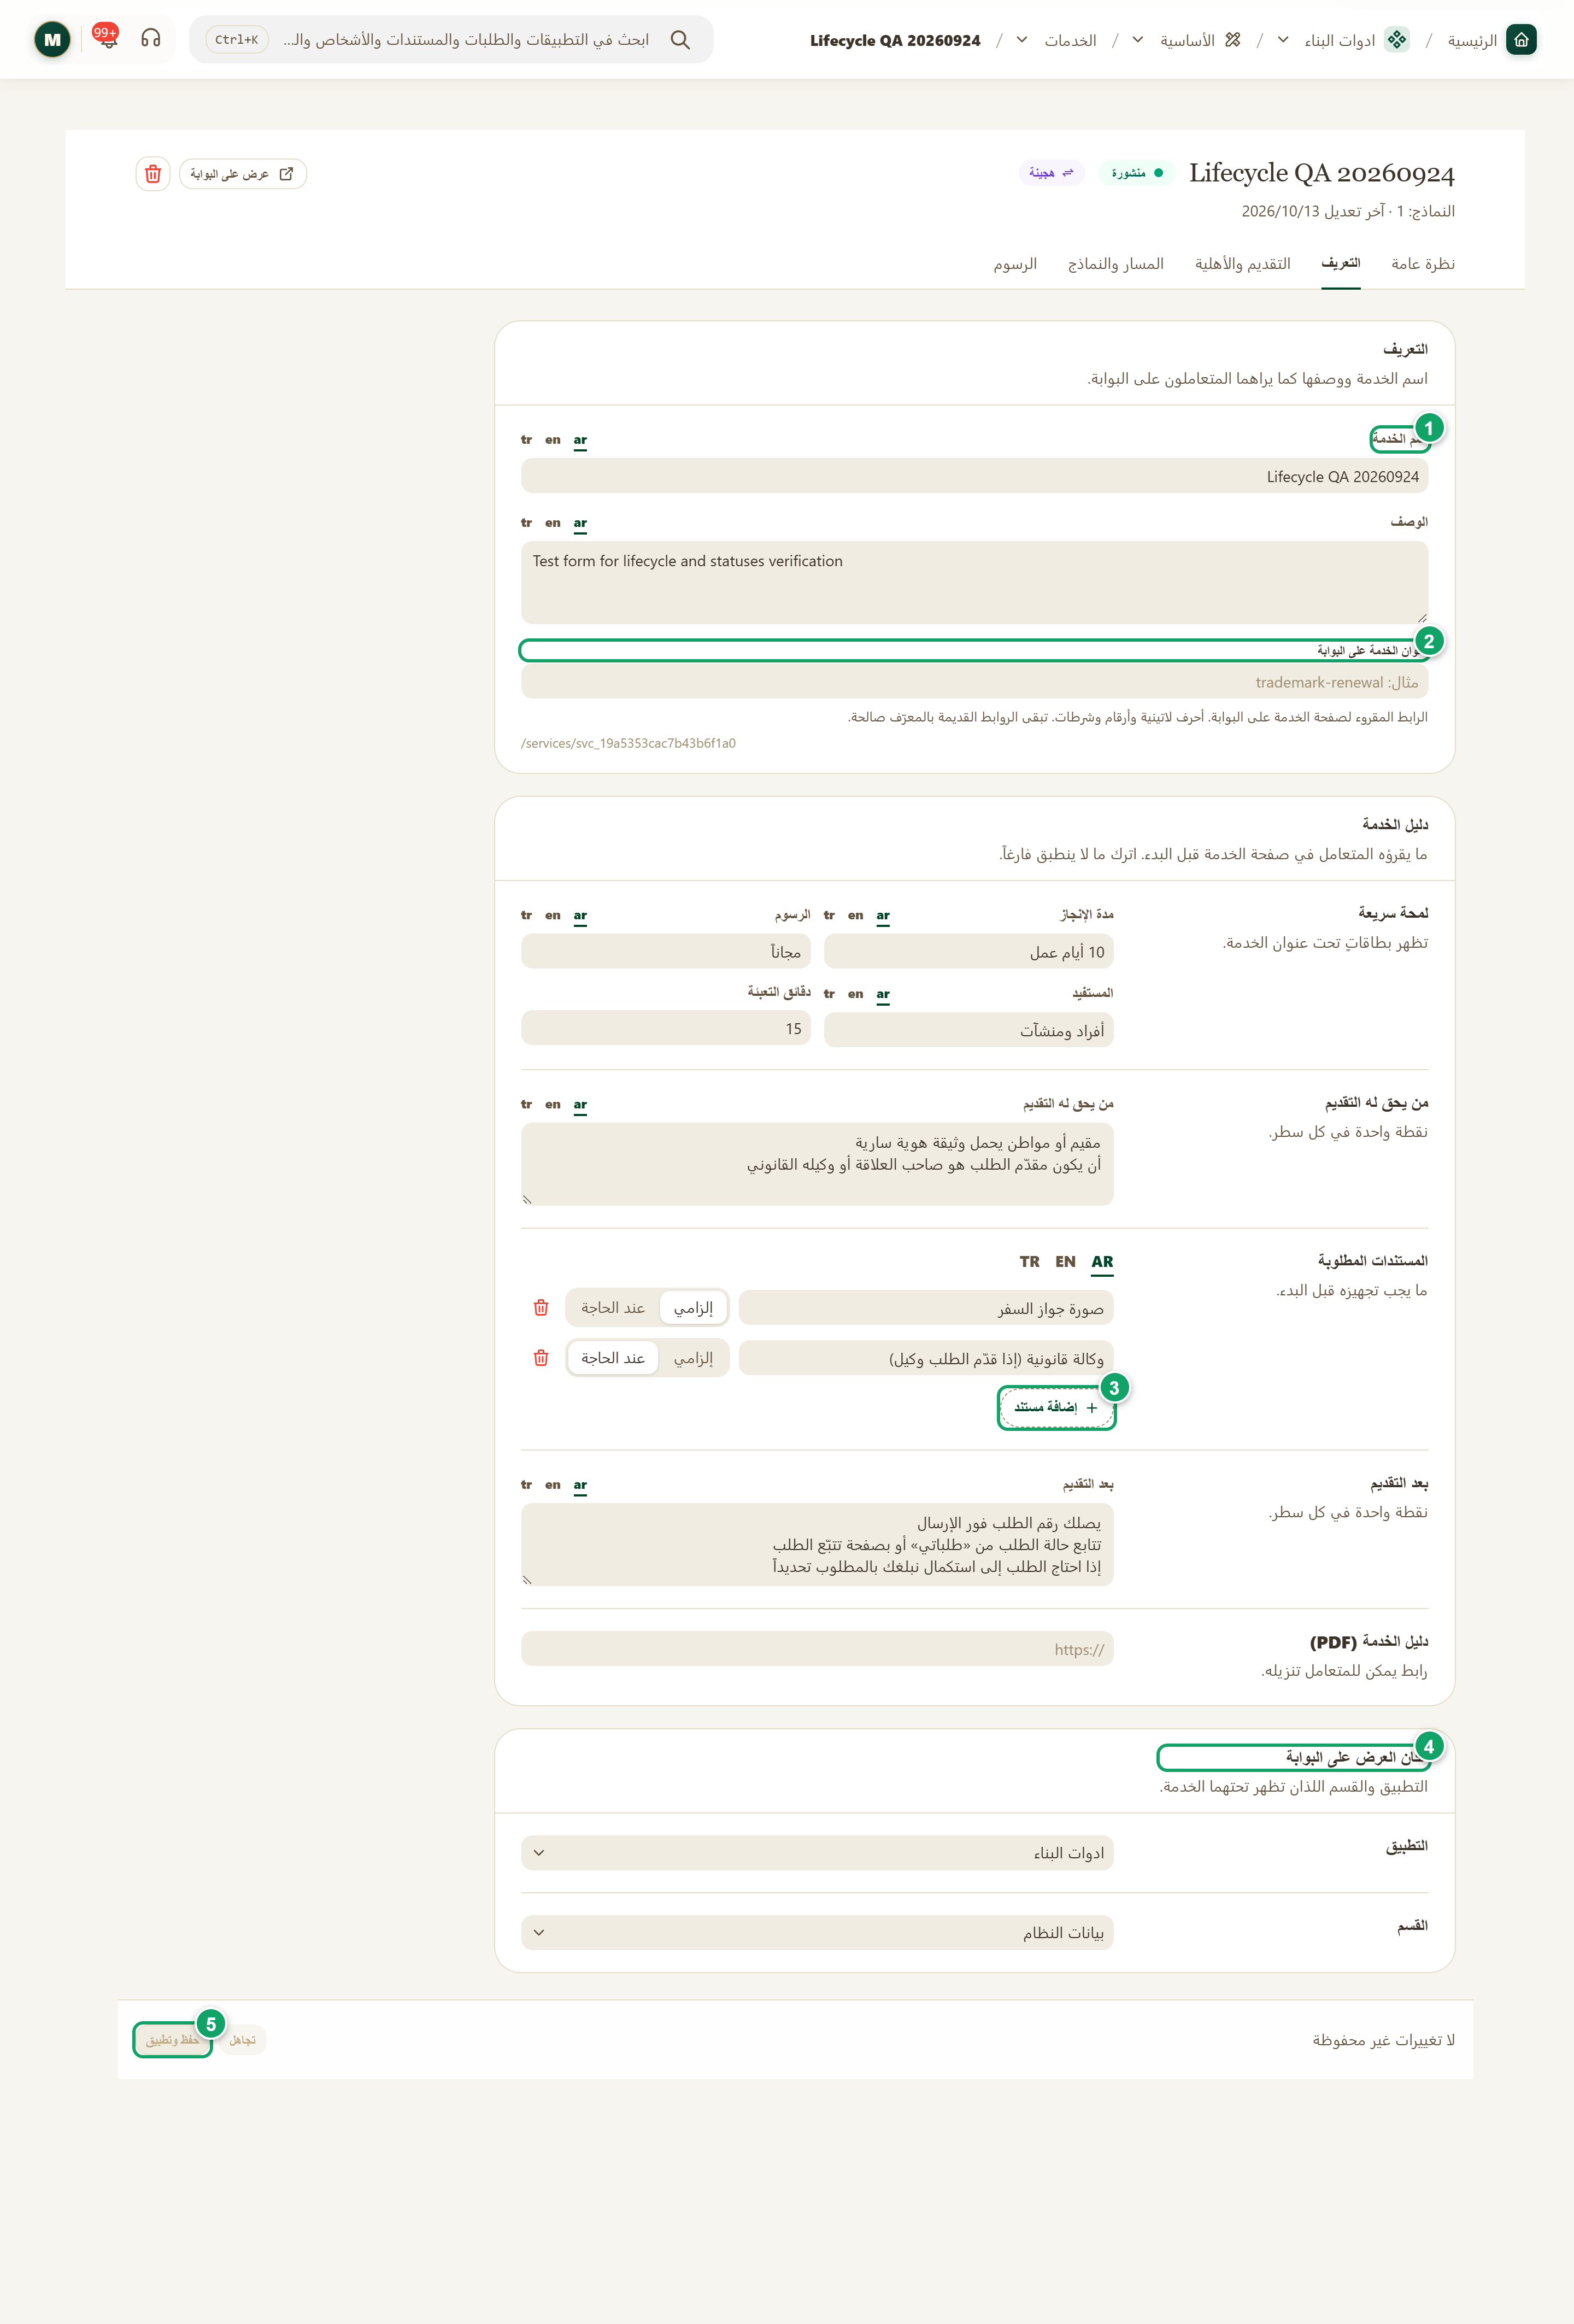
\includegraphics[width=0.95\linewidth,height=0.72\textheight,keepaspectratio]{figures/screens/ch06-services-profile-ar.png}
\caption{تبويب «التعريف» ودليل الخدمة}
\label{fig:builder-services-profile-screen}
\shotnote{تعرض الصورة تبويب «التعريف» لخدمة في مؤسسة الاختبار، وفيها حقول «لمحة سريعة» و«المستندات المطلوبة» ما زالت فارغة. وتوضح أن ما يقرؤه المتعامل قبل أن يبدأ يُكتب كله هنا، ثم يسري على البوابة بزر واحد. ① «اسم الخدمة». ② «عنوان الخدمة على البوابة»: رابط مقروء اختياري لصفحة الخدمة. ③ «إضافة مستند»: يضيف مستنداً مطلوباً وتحدد له «إلزامي» أو «عند الحاجة». ④ «مكان العرض على البوابة»: التطبيق والقسم اللذان تظهر تحتهما الخدمة. ⑤ «حفظ وتطبيق»: يحفظ التعريف ويُعطَّل حتى تغيّر شيئاً.}
\end{figure}

\begin{table}[H]
\centering
\caption{أقسام تبويب «التعريف»}
\label{tab:builder-services-profile-parts}
\begin{tabularx}{\linewidth}{R{3.6cm} Y}
\rcHeaderRow
\thh{القسم} & \thh{ما تكتبه فيه}\\
التعريف & «اسم الخدمة» وهو مطلوب، و«الوصف» الذي يذكر لمن الخدمة وما يحصل عليه المتعامل.\\
عنوان الخدمة على البوابة & الرابط المقروء لصفحة الخدمة، من 3 إلى 80 حرفاً لاتينياً صغيراً أو رقماً مع شرطات، مثل \en{branch-visit}. وتبقى الروابط القديمة بالمعرّف صالحة.\\
دليل الخدمة & «لمحة سريعة» تظهر بطاقاتٍ تحت العنوان: «مدة الإنجاز» و«الرسوم» و«المستفيد» و«دقائق التعبئة». ثم «من يحق له التقديم» و«المستندات المطلوبة» و«بعد التقديم» و«دليل الخدمة (PDF)».\\
مكان العرض على البوابة & «التطبيق» و«القسم» اللذان تظهر تحتهما الخدمة.\\
\end{tabularx}
\end{table}

ولكل مستند في «المستندات المطلوبة» نوع: «إلزامي» أو «عند الحاجة». وتهمّك هذه القائمة لاحقاً، لأن مكتب الاستقبال يعرضها على موظف المركز ليؤشّر ما استلمه من المتعامل. واترك فارغاً ما لا ينطبق على خدمتك.

\begin{figure}[H]
\centering
\begin{tikzpicture}[node distance=0.5cm]
\node[stepBox] (a) {\RL{الاسم والوصف}};
\node[stepBox,below=of a] (b) {\RL{لمحة سريعة}};
\node[stepBox,below=of b] (c) {\RL{المستندات المطلوبة}};
\node[stepBox,below=of c] (d) {\RL{مكان العرض على البوابة}};
\node[stepBox,below=of d] (e) {\RL{حفظ وتطبيق}};
\draw[flowsTo] (a) -- (b);
\draw[flowsTo] (b) -- (c);
\draw[flowsTo] (c) -- (d);
\draw[flowsTo] (d) -- (e);
\end{tikzpicture}
\rclegend
\caption{إكمال تعريف الخدمة}
\label{fig:builder-services-profile-flow}
\shotnote{يرتّب المخطط الأقسام كما يقرؤها المتعامل: الاسم والوصف أولاً، ثم المدة والرسوم، ثم ما يجب أن يجهّزه. وينتهي بالحفظ لأن التغييرات تسري على البوابة فوره، دون إعادة نشر أي نموذج.}
\end{figure}

\subsection{خطوات العمل والتحقق}
\begin{enumerate}
\item افتح الخدمة واضغط تبويب «التعريف».
\item اكتب «اسم الخدمة» و«الوصف»، وأضف «عنوان الخدمة على البوابة» إن أردت رابطاً مقروءاً.
\item املأ «لمحة سريعة»، ثم أضف المستندات بزر «إضافة مستند» وحدد لكل منها «إلزامي» أو «عند الحاجة».
\item اختر «التطبيق» و«القسم» في «مكان العرض على البوابة»، ثم اضغط «حفظ وتطبيق».
\end{enumerate}

\textbf{تحقق ومعالجة المشكلة:} يتغير شريط الحفظ إلى «لا تغييرات غير محفوظة»، ويصبح بند «الملف التعريفي والدليل» مكتملاً في «نظرة عامة». فإذا بقي زر الحفظ معطلاً، فتحقق من أن «اسم الخدمة» غير فارغ وأن العنوان يطابق الشرط المكتوب تحته. وإذا ظهر «هذا العنوان مستخدم لخدمة أخرى.»، فاختر عنواناً مختلفاً.

\clearpage
\section{التقديم والأهلية}
\label{sec:builder-feature-services-delivery}

يحدد تبويب «التقديم والأهلية» كيف تُقدَّم الخدمة، ومتى تكون متاحة، ومن يحق له التقديم وبأي شروط. وبذلك يمنع الطلبات التي لا تستوفي الشروط قبل أن تبدأ، بدلاً من رفضها بعد وصولها. وتختلف الأقسام الظاهرة بحسب طريقة التقديم: فالخدمة التي تبدأ عبر البوابة تعرض أقسام الأهلية والتحقق، والخدمة التي فيها خطوات حضورية تعرض مراكز الخدمة والمواعيد والاستقبال.

\textbf{المسار ومن يستخدمه:} «الخدمات» ← اضغط الخدمة ← «التقديم والأهلية». يضبطه من يبني الخدمة، ويعود إليه لإغلاقها مؤقتاً أو لتغيير شروطها.

\begin{rcnote}[مثال: شركة الأفق]
يختار مسؤول النظام لخدمة «طلب زيارة فرع» «أصحاب الحسابات المسجّلة فقط» ③، ويحدد «الطلبات المفتوحة لكل متعامل» بطلب واحد حتى لا يكرر العميل الطلب نفسه. ثم يختار فرع حلب في «مراكز الخدمة» ويفعّل «الاستقبال في المركز».
\end{rcnote}

\begin{figure}[H]
\centering
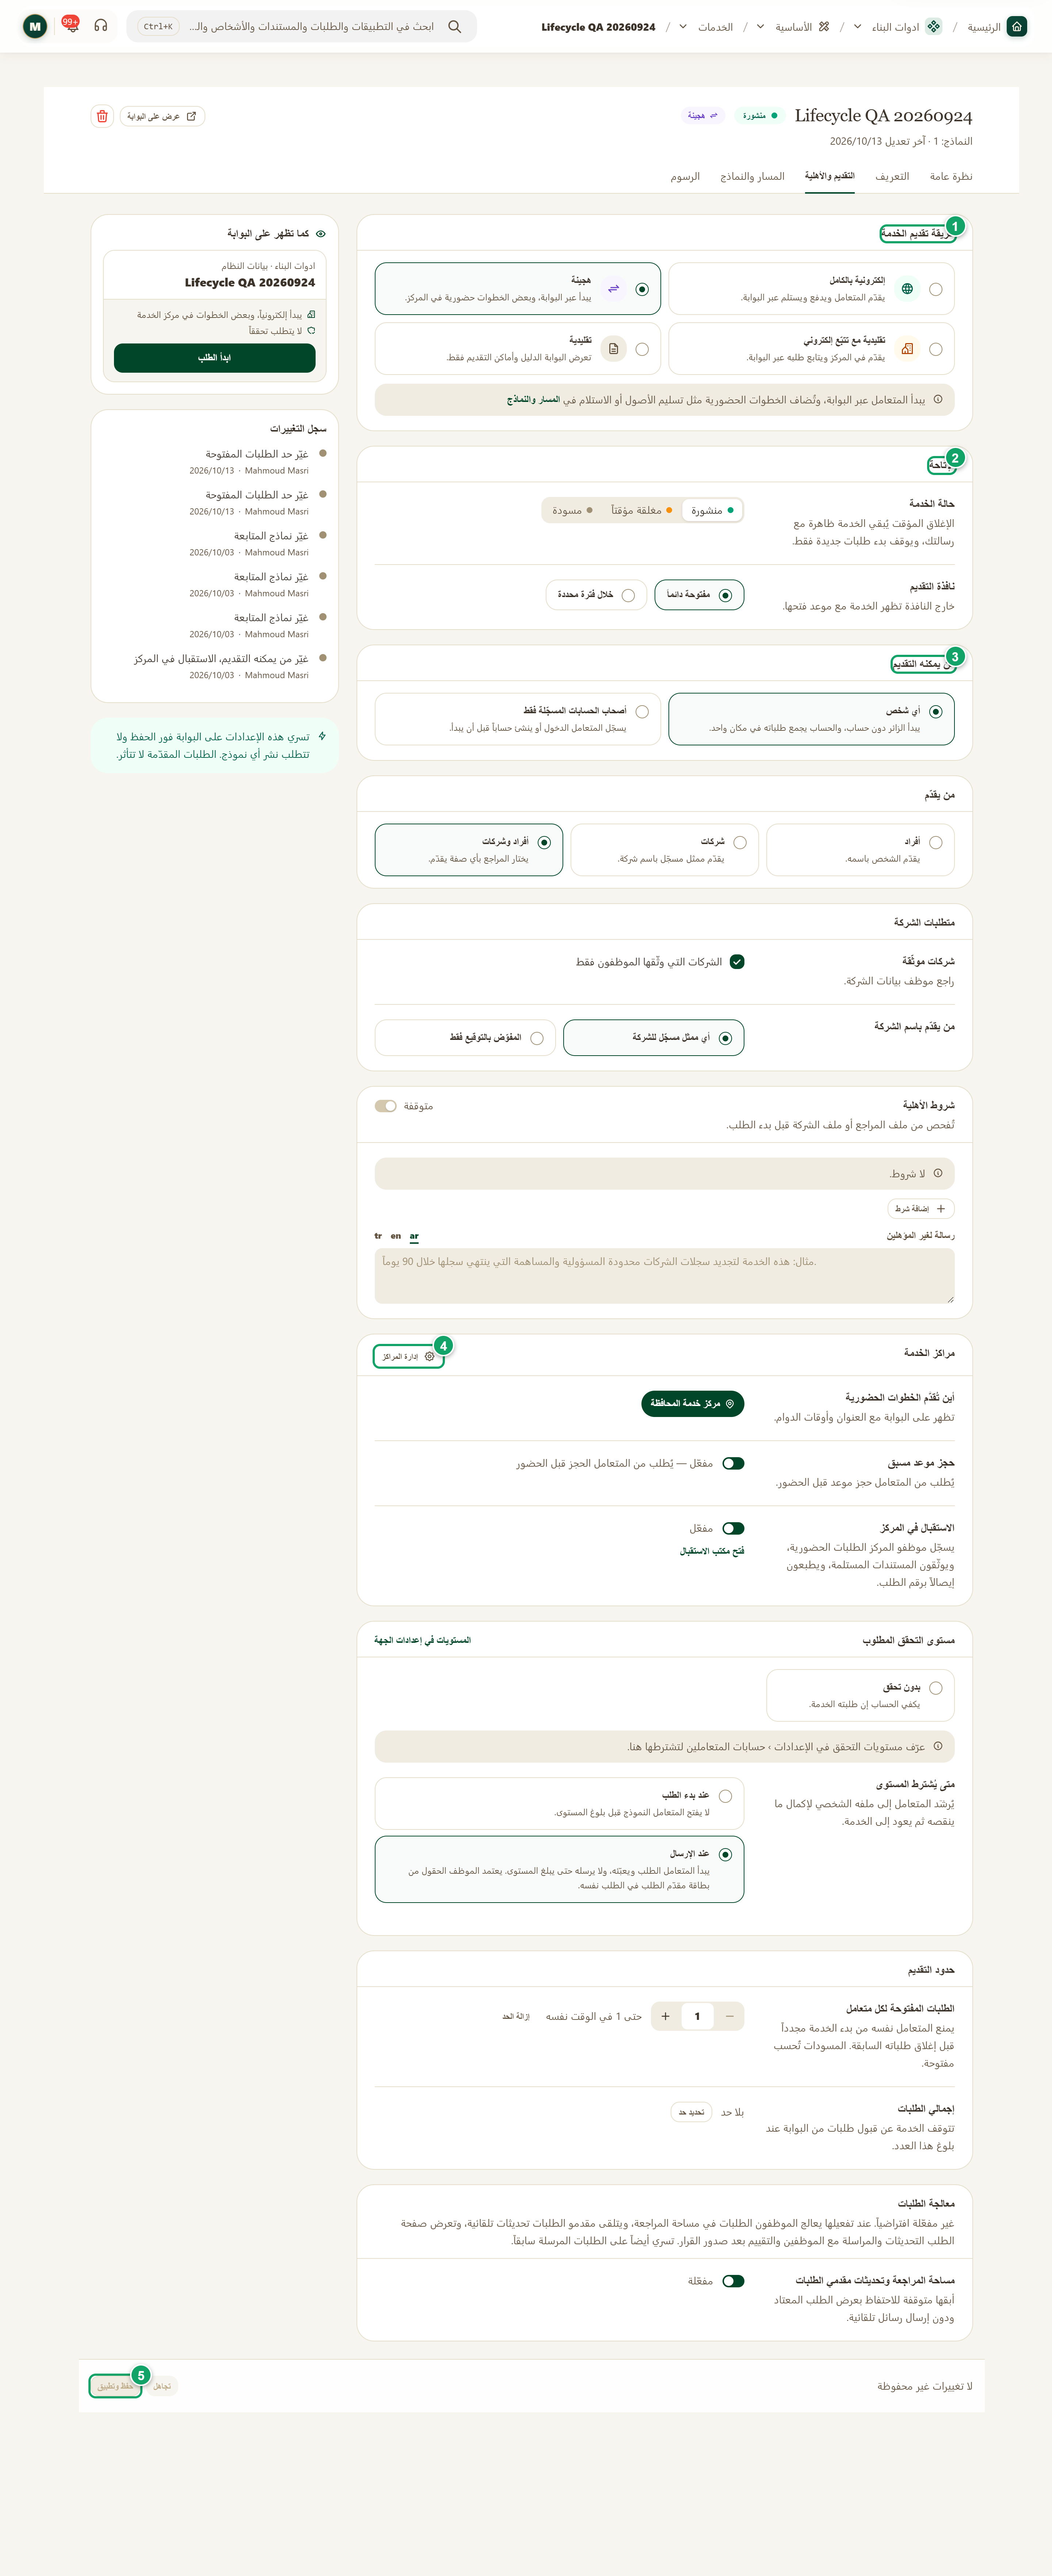
\includegraphics[width=0.95\linewidth,height=0.72\textheight,keepaspectratio]{figures/screens/ch06-services-delivery-ar.png}
\caption{تبويب «التقديم والأهلية» لخدمة هجينة}
\label{fig:builder-services-delivery-screen}
\shotnote{تعرض الصورة تبويب «التقديم والأهلية» لخدمة هجينة في مؤسسة الاختبار، لذلك يجمع أقسام الأهلية والتحقق التي تخص البدء عبر البوابة وأقسام المراكز والاستقبال التي تخص الخطوات الحضورية. وتبيّن أن الأقسام تُقرأ من الأعلى إلى الأسفل بالترتيب الذي تُضبط به، ثم تُحفظ معاً. ① «طريقة تقديم الخدمة»: الطرق الأربع، وهي التي تحدد الأقسام الظاهرة بعدها. ② «الإتاحة»: حالة الخدمة ونافذة التقديم. ③ «من يمكنه التقديم»: أي شخص أو أصحاب الحسابات المسجّلة فقط. ④ «إدارة المراكز»: يفتح نافذة «مراكز الخدمة». ⑤ «حفظ وتطبيق»: يطبّق الإعدادات على البوابة فوراً.}
\end{figure}

\begin{table}[H]
\centering
\caption{أقسام التقديم والإتاحة}
\label{tab:builder-services-delivery-parts}
\begin{tabularx}{\linewidth}{R{3.6cm} Y}
\rcHeaderRow
\thh{القسم} & \thh{ما تضبطه فيه}\\
طريقة تقديم الخدمة & إحدى الطرق الأربع. وإذا لم يناسب المسار الحالي الطريقة الجديدة، يظهر زر «تعديل المسار»، ولا تُطبَّق الطريقة إلا بعد حفظ المسار المعدّل.\\
الإتاحة & «حالة الخدمة»: «منشورة» أو «مغلقة مؤقتاً» مع «رسالة للمتعاملين» أو «مسودة». و«نافذة التقديم»: «مفتوحة دائماً» أو «خلال فترة محددة» بتاريخين.\\
من يمكنه التقديم & للخدمات التي تبدأ عبر البوابة: «أي شخص» دون حساب، أو «أصحاب الحسابات المسجّلة فقط».\\
مستوى التحقق المطلوب & للخدمات التي تبدأ عبر البوابة: «بدون تحقق» أو أحد المستويات المعرّفة في الإعدادات، ثم «متى يُشترط المستوى»: «عند بدء الطلب» أو «عند الإرسال».\\
حدود التقديم & «الطلبات المفتوحة لكل متعامل» حتى 9 طلبات، و«إجمالي الطلبات» الذي تتوقف الخدمة بعده عن قبول طلبات البوابة.\\
مراكز الخدمة وحجز موعد مسبق & للخدمات التي فيها خطوات حضورية: المراكز التي تجري فيها، وهل يُطلب من المتعامل «حجز موعد مسبق».\\
الاستقبال في المركز & يسمح لموظفي المركز بتسجيل الطلبات الحضورية وطباعة إيصال، ومنه رابط «فتح مكتب الاستقبال».\\
معالجة الطلبات & «مساحة المراجعة وتحديثات مقدمي الطلبات»: غير مفعّلة افتراضياً، وعند تفعيلها يعالج الموظفون الطلبات في مساحة المراجعة ويتلقى مقدمو الطلبات تحديثات تلقائية.\\
\end{tabularx}
\end{table}

\begin{table}[H]
\centering
\caption{أقسام الأهلية للخدمات التي تبدأ عبر البوابة}
\label{tab:builder-services-delivery-eligibility}
\begin{tabularx}{\linewidth}{R{3.6cm} Y}
\rcHeaderRow
\thh{القسم} & \thh{ما تضبطه فيه}\\
من يقدّم & «أفراد» أو «شركات» أو «أفراد وشركات». ويتطلب خيارا الشركات تفعيل ملفات الشركات من «إعدادات ملف الشركة».\\
متطلبات الشركة & «الشركات التي وثّقها الموظفون فقط»، و«من يقدّم باسم الشركة»: «أي ممثل مسجّل للشركة» أو «المفوّض بالتوقيع فقط».\\
شروط الأهلية & تفعّلها بـ«استخدام شروط الأهلية»، ثم تضيف بزر «إضافة شرط» شروطاً تُفحص من ملف المراجع أو ملف الشركة قبل بدء الطلب، مثل «العمر لا يقل عن». وتكتب «رسالة لغير المؤهلين».\\
\end{tabularx}
\end{table}

\begin{rcwarn}[مستوى يعتمده الموظف لا يُشترط عند البدء]
إذا تضمّن المستوى المختار حقلاً يعتمده الموظف من طلب قائم، واشترطته «عند بدء الطلب»، فلن يتمكن متعامل جديد من بدء الخدمة أبداً. لذلك يظهر تحذير مع زر «اشترطه عند الإرسال»، فاضغطه قبل الحفظ.
\end{rcwarn}

\begin{figure}[H]
\centering
\begin{tikzpicture}[node distance=0.5cm]
\node[stepBox] (a) {\RL{طريقة تقديم الخدمة}};
\node[stepBox,below=of a] (b) {\RL{الإتاحة}};
\node[stepBox,below=of b] (c) {\RL{من يقدّم وشروطه}};
\node[stepBox,below=of c] (d) {\RL{المراكز والاستقبال}};
\node[stepBox,below=of d] (e) {\RL{حفظ وتطبيق}};
\draw[flowsTo] (a) -- (b);
\draw[flowsTo] (b) -- (c);
\draw[flowsTo] (c) -- (d);
\draw[flowsTo] (d) -- (e);
\end{tikzpicture}
\rclegend
\caption{ضبط التقديم والأهلية}
\label{fig:builder-services-delivery-flow}
\shotnote{تأتي طريقة التقديم أولاً لأنها تحدد الأقسام التي تظهر بعدها: أقسام الأهلية والتحقق للخدمات التي تبدأ عبر البوابة، وأقسام المراكز والاستقبال للخدمات التي فيها خطوات حضورية. وتسري الإعدادات كلها على البوابة فور الحفظ، ولا تتأثر الطلبات المقدّمة قبلها.}
\end{figure}

\subsection{خطوات العمل والتحقق}
\begin{enumerate}
\item افتح الخدمة واضغط «التقديم والأهلية»، ثم تأكد من «طريقة تقديم الخدمة».
\item اختر في «الإتاحة» «حالة الخدمة» و«نافذة التقديم».
\item حدد «من يمكنه التقديم» و«من يقدّم»، وأضف «شروط الأهلية» إن احتجت إليها.
\item اختر مراكز الخدمة وفعّل «الاستقبال في المركز» إن كانت للخدمة خطوات حضورية، ثم اضبط «حدود التقديم».
\item اضغط «حفظ وتطبيق».
\end{enumerate}

\textbf{تحقق ومعالجة المشكلة:} تظهر رسالة «حُفظت — تسري على البوابة الآن»، وتتغير معاينة «كما تظهر على البوابة» بحسب اختياراتك. فإذا بقي زر الحفظ معطلاً بعد تغيير الطريقة، فاضغط «تعديل المسار» واحفظ المسار المناسب لها. وإذا ظهر «يجب أن تنتهي النافذة بعد بدايتها.»، فصحّح تاريخ «إلى».

\clearpage
\section{مراكز الخدمة}
\label{sec:builder-feature-services-centers}

مراكز الخدمة هي الأماكن التي يحضر إليها المتعاملون للخطوات الحضورية، مثل تسليم الأصول أو استلام النتيجة. وتُعرَّف المراكز مرة واحدة للمؤسسة كلها، ثم تختار كل خدمة منها ما يناسبها، فتظهر على البوابة مع العنوان وأوقات الدوام. ويحدد كل مركز أيضاً الموظفين الذين يفتح لهم مكتب الاستقبال عليه.

\textbf{المسار ومن يستخدمه:} «الخدمات» ← اضغط خدمة طريقتها ليست «إلكترونية بالكامل» ← «التقديم والأهلية» ← «إدارة المراكز». يضبطها مسؤول الخدمات عند افتتاح مركز أو تغيير دوامه أو موظفيه.

\begin{rcnote}[مثال: شركة الأفق]
يضيف مسؤول النظام بزر «إضافة مركز» ① مركزاً باسم «فرع حلب» ② وآخر باسم «المقر الرئيسي، دمشق» مع عنوان كل منهما وأوقات الدوام. ثم يضيف عمر حداد إلى «موظفو هذا المركز» ③ في فرع حلب، فيفتح مكتب الاستقبال لديه على هذا الفرع.
\end{rcnote}

\begin{figure}[H]
\centering
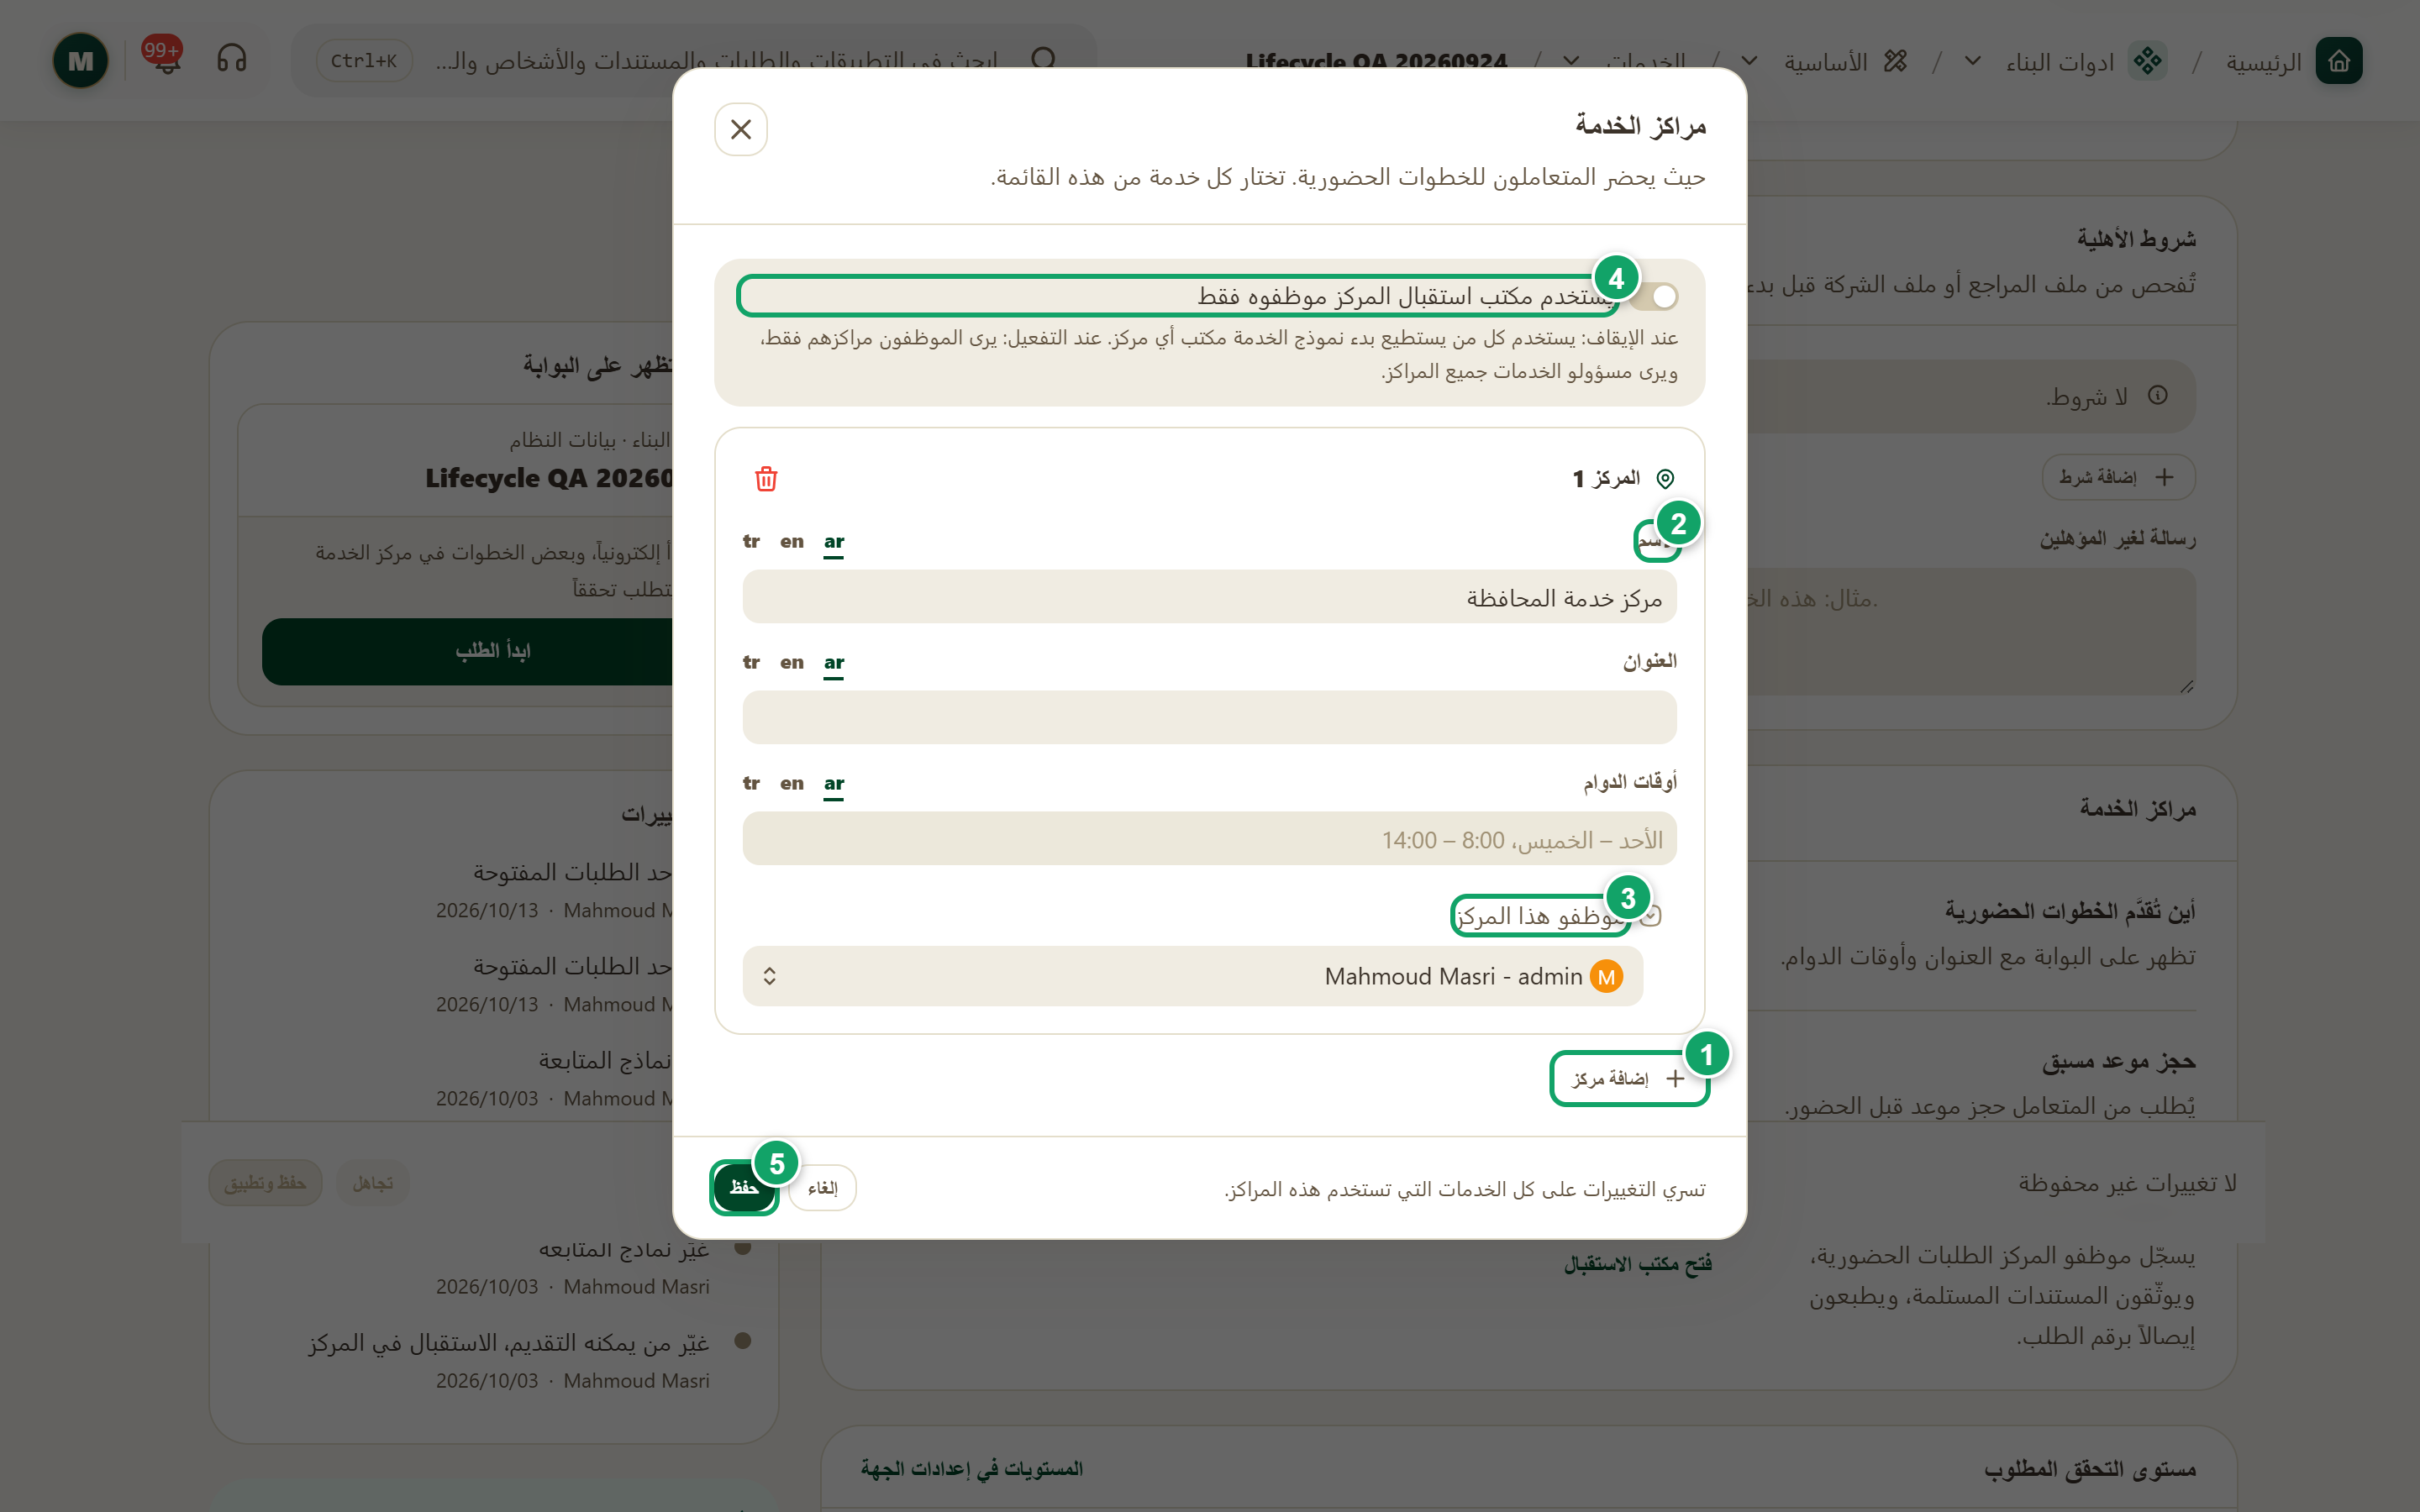
\includegraphics[width=0.95\linewidth,height=0.72\textheight,keepaspectratio]{figures/screens/ch06-services-centers-ar.png}
\caption{نافذة «مراكز الخدمة»}
\label{fig:builder-services-centers-screen}
\shotnote{تعرض الصورة نافذة «مراكز الخدمة» في مؤسسة الاختبار وفيها مركز واحد له اسم وأوقات دوام وموظف واحد. وتذكّرك العبارة أسفل النافذة بأن التغييرات تسري على كل الخدمات التي تستخدم هذه المراكز، لا على الخدمة المفتوحة وحدها. ① «إضافة مركز». ② «الاسم»: اسم المركز المطلوب كما يظهر للمتعاملين. ③ «موظفو هذا المركز»: من يفتح لهم مكتب الاستقبال على هذا المركز. ④ «يستخدم مكتب استقبال المركز موظفوه فقط»: يقصر مكتب كل مركز على موظفيه. ⑤ «حفظ»: يحفظ المراكز للمؤسسة كلها.}
\end{figure}

\begin{table}[H]
\centering
\caption{ما تضبطه في نافذة «مراكز الخدمة»}
\label{tab:builder-services-centers-parts}
\begin{tabularx}{\linewidth}{R{3.6cm} Y}
\rcHeaderRow
\thh{الحقل أو الخيار} & \thh{ما يعنيه}\\
الاسم & اسم المركز كما يظهر للمتعاملين، وهو مطلوب.\\
العنوان وأوقات الدوام & يظهران على البوابة، مثل «الأحد – الخميس، 8:00 – 14:00»، ويُطبع الدوام على إيصال الطلب الحضوري.\\
موظفو هذا المركز & الموظفون الذين يفتح مكتب الاستقبال لديهم على هذا المركز.\\
يستخدم مكتب استقبال المركز موظفوه فقط & عند الإيقاف يستخدم كل من يستطيع بدء نموذج الخدمة مكتب أي مركز. وعند التفعيل يرى الموظفون مراكزهم فقط، ويرى مسؤولو الخدمات جميع المراكز.\\
\end{tabularx}
\end{table}

\begin{rcwarn}[التغيير يشمل كل الخدمات]
تسري تغييرات المراكز على كل الخدمات التي تستخدمها، لذلك لا تحذف مركزاً أو تغيّر دوامه إلا بعد التأكد من الخدمات المرتبطة به.
\end{rcwarn}

\begin{figure}[H]
\centering
\begin{tikzpicture}[node distance=0.5cm]
\node[stepBox] (a) {\RL{إدارة المراكز}};
\node[stepBox,below=of a] (b) {\RL{إضافة مركز وبياناته}};
\node[stepBox,below=of b] (c) {\RL{تحديد موظفي المركز}};
\node[stepBox,below=of c] (d) {\RL{اختياره في الخدمة}};
\node[stepBox,below=of d] (e) {\RL{حفظ وتطبيق}};
\draw[flowsTo] (a) -- (b);
\draw[flowsTo] (b) -- (c);
\draw[flowsTo] (c) -- (d);
\draw[flowsTo] (d) -- (e);
\end{tikzpicture}
\rclegend
\caption{إعداد مركز خدمة وربطه بالخدمة}
\label{fig:builder-services-centers-flow}
\shotnote{يفصل المخطط بين خطوتين تُحفظ كل منهما وحدها: النافذة تحفظ المراكز للمؤسسة كلها بزر «حفظ»، ثم تختار الخدمة مراكزها وتحفظها بزر «حفظ وتطبيق». فإنشاء المركز وحده لا يجعله ظاهراً في خدمة بعينها.}
\end{figure}

\subsection{خطوات العمل والتحقق}
\begin{enumerate}
\item افتح «التقديم والأهلية» في خدمة لها خطوات حضورية، واضغط «إدارة المراكز».
\item اضغط «إضافة مركز»، واكتب «الاسم» و«العنوان» و«أوقات الدوام».
\item اختر «موظفو هذا المركز»، وقرّر هل تفعّل «يستخدم مكتب استقبال المركز موظفوه فقط»، ثم اضغط «حفظ».
\item اختر المركز في «أين تُقدَّم الخطوات الحضورية»، ثم اضغط «حفظ وتطبيق».
\end{enumerate}

\textbf{تحقق ومعالجة المشكلة:} يظهر المركز في معاينة «كما تظهر على البوابة» وفي بطاقة «مراكز الخدمة» في «نظرة عامة». وإذا ظهر للموظف في مكتب الاستقبال «لست ضمن موظفي أي مركز خدمة»، فأضفه إلى «موظفو هذا المركز». وإذا لم يُحفظ المركز، فتحقق من أن لكل مركز اسماً.

\clearpage
\section{المسار والنماذج}
\label{sec:builder-feature-services-path}

يرسم تبويب «المسار والنماذج» ما يمر به الطلب بالترتيب: خطوة البدء، ثم الخطوات التالية، وأين تجري كل منها. فقد تكون الخطوة نموذجاً يعبّئه المتعامل عبر البوابة، أو خطوة حضورية في المركز يوثّقها الموظف. ويضم التبويب أيضاً النماذج التي يبدؤها المتعامل في أي وقت خارج المسار، ونماذج المتابعة التي تُطلب منه عند حالة معينة.

\textbf{المسار ومن يستخدمه:} «الخدمات» ← اضغط الخدمة ← «المسار والنماذج». يبنيه مسؤول الخدمة بعد نشر النماذج التي سيستخدمها.

\begin{rcnote}[مثال: شركة الأفق]
يبدأ مسار «طلب زيارة فرع» بنموذج الطلب عبر البوابة، ثم يضيف مسؤول النظام بزر «إضافة خطوة» ① خطوة حضورية باسم «حضور الزيارة» ② تُتاح عندما يكون الطلب «مقبول». ويفعّل لها «يتطلب موعداً»، فتظهر عليها شارة «بموعد».
\end{rcnote}

\begin{figure}[H]
\centering
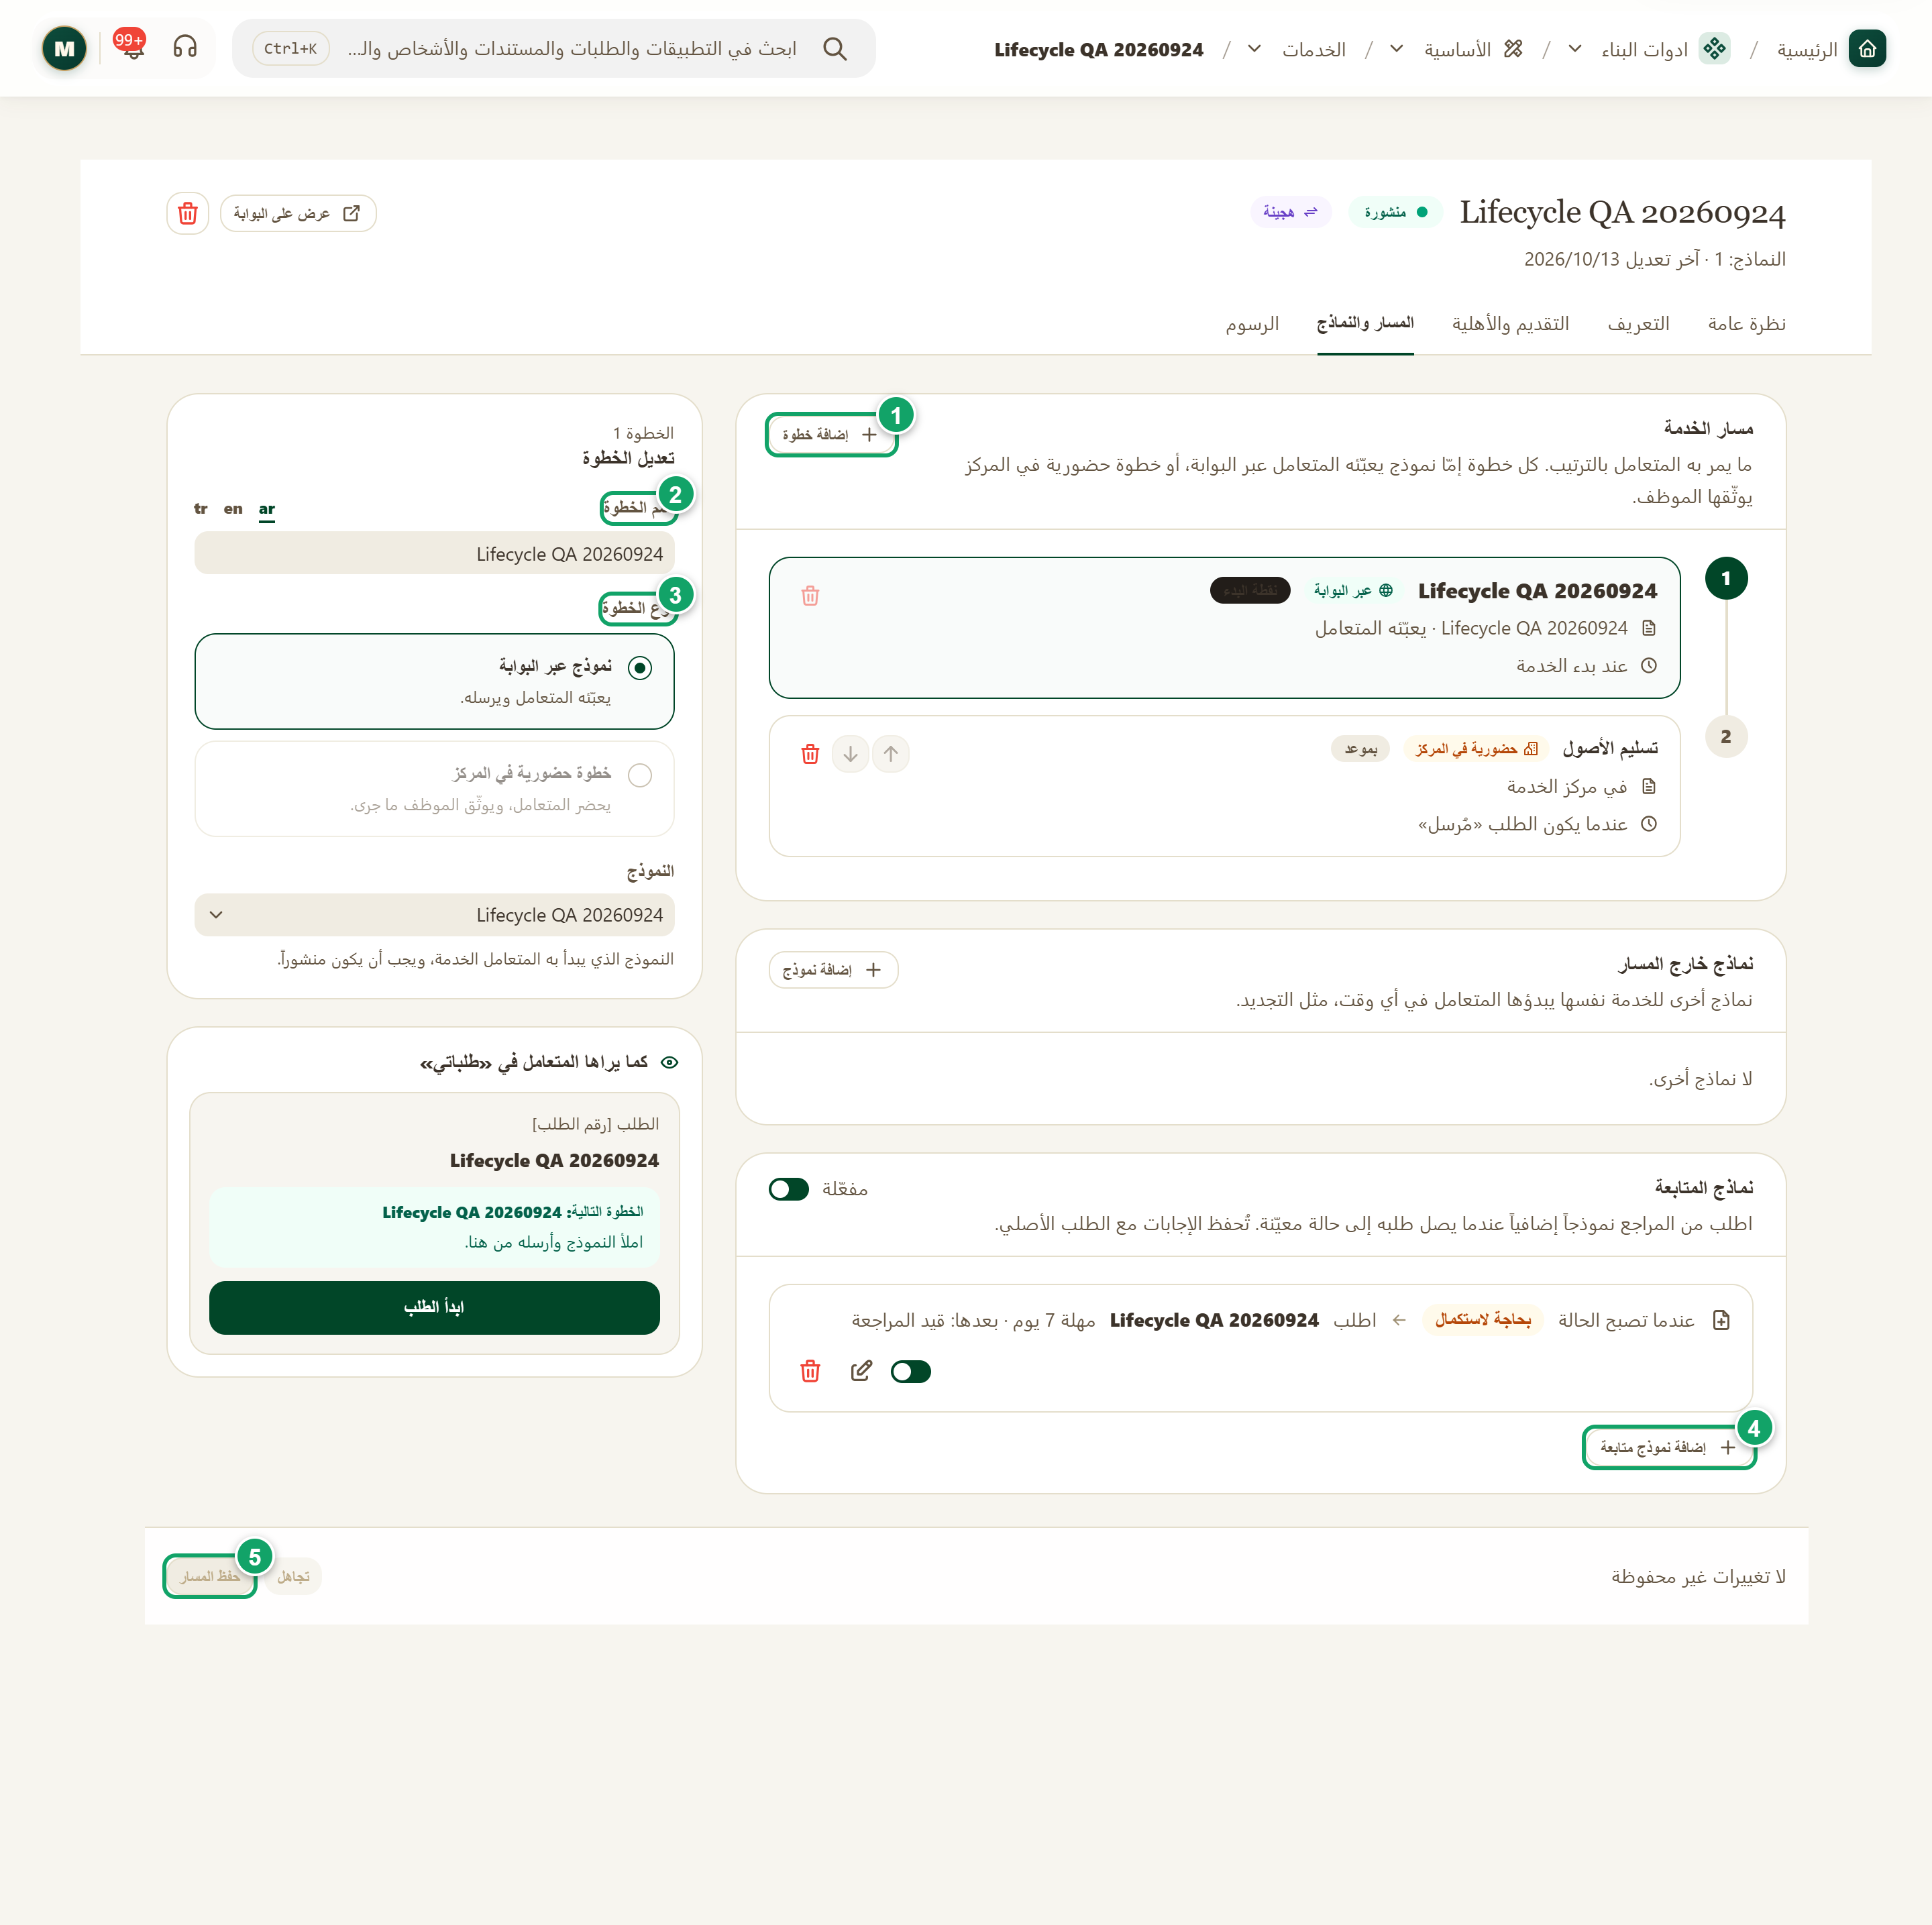
\includegraphics[width=0.95\linewidth,height=0.72\textheight,keepaspectratio]{figures/screens/ch06-services-path-ar.png}
\caption{تبويب «المسار والنماذج»}
\label{fig:builder-services-path-screen}
\shotnote{تعرض الصورة مسار خدمة هجينة في مؤسسة الاختبار: خطوة البدء عبر البوابة بشارة «نقطة البدء»، ثم خطوة حضورية «بموعد»، ومعهما قاعدة متابعة واحدة. وتبيّن أن الخطوة المختارة تُعدَّل في اللوحة الجانبية، وأن خيار الخطوة الحضورية معطّل لخطوة البدء في هذه الطريقة. ① «إضافة خطوة»: يضيف خطوة في آخر المسار. ② «اسم الخطوة»: الاسم الذي يراه المتعامل في «طلباتي». ③ «نوع الخطوة»: نموذج عبر البوابة أو خطوة حضورية في المركز. ④ «إضافة نموذج متابعة»: يضيف قاعدة تطلب نموذجاً عند حالة معينة. ⑤ «حفظ المسار».}
\end{figure}

\begin{table}[H]
\centering
\caption{إعدادات الخطوة}
\label{tab:builder-services-path-step}
\begin{tabularx}{\linewidth}{R{3.6cm} Y}
\rcHeaderRow
\thh{الإعداد} & \thh{ما يعنيه}\\
اسم الخطوة & الاسم الذي يراه المتعامل في «طلباتي»، مثل «الخطوة التالية: …».\\
نوع الخطوة & «نموذج عبر البوابة» يعبّئه المتعامل ويرسله، أو «خطوة حضورية في المركز» يحضر لها المتعامل ويوثّق الموظف ما جرى.\\
النموذج أو محضر الموظف & لخطوة البوابة نموذج منشور، ويمكن تركه فارغاً إذا استُكملت الخطوة في الطلب نفسه. وللخطوة الحضورية «محضر الموظف (اختياري)».\\
متى تُتاح & «بعد الخطوة السابقة»، أو عندما يصل الطلب إلى حالة من حالات نموذج البدء.\\
يتطلب موعداً & للخطوات الحضورية، ويعني أن يحجز المتعامل موعداً في أحد مراكز الخدمة.\\
\end{tabularx}
\end{table}

وتحمل الخطوة الأولى شارة «نقطة البدء»، ولا يمكن حذفها في الخدمات التي تبدأ عبر البوابة. وتضم الخدمة حتى 20 خطوة، ولا يتكرر النموذج فيها. أما الخدمة «إلكترونية بالكامل» فلا تضم خطوات حضورية، والخدمة التقليدية تبدأ خطوتها الأولى في المركز.

\begin{table}[H]
\centering
\caption{أقسام التبويب الأخرى}
\label{tab:builder-services-path-more}
\begin{tabularx}{\linewidth}{R{3.6cm} Y}
\rcHeaderRow
\thh{القسم} & \thh{ما يقدمه}\\
نماذج خارج المسار & للخدمات التي تبدأ عبر البوابة: نماذج منشورة يبدؤها المتعامل في أي وقت، مثل التجديد، وتضيفها بزر «إضافة نموذج».\\
نماذج المتابعة & تفعّلها بـ«استخدام نماذج المتابعة»، ثم تضيف قاعدة: «الحالة التي تطلب النموذج»، و«النموذج»، و«أيام لتعبئته»، و«بعد إرسال المراجع انقل الطلب إلى»، و«أبلغ المراجع». وتُحفظ الإجابات مع الطلب الأصلي.\\
كما يراها المتعامل في «طلباتي» & معاينة للخطوة المختارة كما تظهر للمتعامل في طلبه.\\
\end{tabularx}
\end{table}

\begin{figure}[H]
\centering
\begin{tikzpicture}[node distance=0.5cm]
\node[stepBox] (a) {\RL{نقطة البدء}};
\node[stepBox,below=of a] (b) {\RL{إضافة خطوة}};
\node[stepBox,below=of b] (c) {\RL{نوع الخطوة ونموذجها}};
\node[stepBox,below=of c] (d) {\RL{متى تُتاح}};
\node[stepBox,below=of d] (e) {\RL{حفظ المسار}};
\draw[flowsTo] (a) -- (b);
\draw[flowsTo] (b) -- (c);
\draw[flowsTo] (c) -- (d);
\draw[flowsTo] (d) -- (e);
\end{tikzpicture}
\rclegend
\caption{بناء مسار الخدمة}
\label{fig:builder-services-path-flow}
\shotnote{يبدأ المسار دائماً من نقطة البدء التي حُددت عند إنشاء الخدمة، ثم تُضاف الخطوات بعدها واحدة واحدة. وتعتمد خطوة «متى تُتاح» على حالات نموذج البدء، لذلك اضبط دورة حياته قبل أن تبني مساراً ينتظر حالة معينة.}
\end{figure}

\subsection{خطوات العمل والتحقق}
\begin{enumerate}
\item افتح الخدمة واضغط «المسار والنماذج»، وراجع خطوة «نقطة البدء».
\item اضغط «إضافة خطوة»، واكتب «اسم الخطوة» واختر «نوع الخطوة».
\item اختر «النموذج» أو «محضر الموظف (اختياري)»، ثم حدد «متى تُتاح»، وفعّل «يتطلب موعداً» إن لزم.
\item رتّب الخطوات بزرّي «نقل للأعلى» و«نقل للأسفل»، وأضف نماذج المتابعة إن احتجت إليها.
\item اضغط «حفظ المسار».
\end{enumerate}

\textbf{تحقق ومعالجة المشكلة:} يتحول شريط الحفظ إلى «لا تغييرات غير محفوظة»، ويظهر عدد الخطوات في «جاهزية الخدمة». فإذا عُطّل الحفظ وظهرت رسالة مثل «الخدمة الإلكترونية بالكامل لا تضم خطوات حضورية.»، فغيّر نوع الخطوة أو طريقة التقديم. وإذا ظهر «لا حالات لنموذج البدء بعد»، فأضف الحالات من «دورة الحياة» في النموذج.

\clearpage
\section{الرسوم}
\label{sec:builder-feature-services-fees}

يحوّل تبويب «الرسوم» كلفة الخدمة إلى بنود واضحة، فتعرضها البوابة للمتعامل قبل أن يبدأ، ويعرف كل طلب ما عليه ومتى يُستحق. ويمكن أن يتوقف البند على إجابة في النموذج، وأن يُعفى منه من يقدّم إثباتاً. ويحدد التبويب أيضاً ما يحدث للطلب عندما يُستحق رسم، ومهلة السداد.

\textbf{المسار ومن يستخدمه:} «الخدمات» ← اضغط الخدمة ← «الرسوم». يضبطه من يبني الخدمة بالتنسيق مع المسؤول المالي.

\begin{rcnote}[مثال: شركة الأفق]
يفعّل مسؤول النظام «استخدام بنود الرسوم»، ويضيف بزر «إضافة بند» ① بنداً باسم «رسم الزيارة» يُستحق «عند زيارة المركز». فيرى العميل الرسم على صفحة الخدمة، ويسجّل عمر حداد رقم الإيصال عند استلامه في فرع حلب.
\end{rcnote}

\begin{figure}[H]
\centering
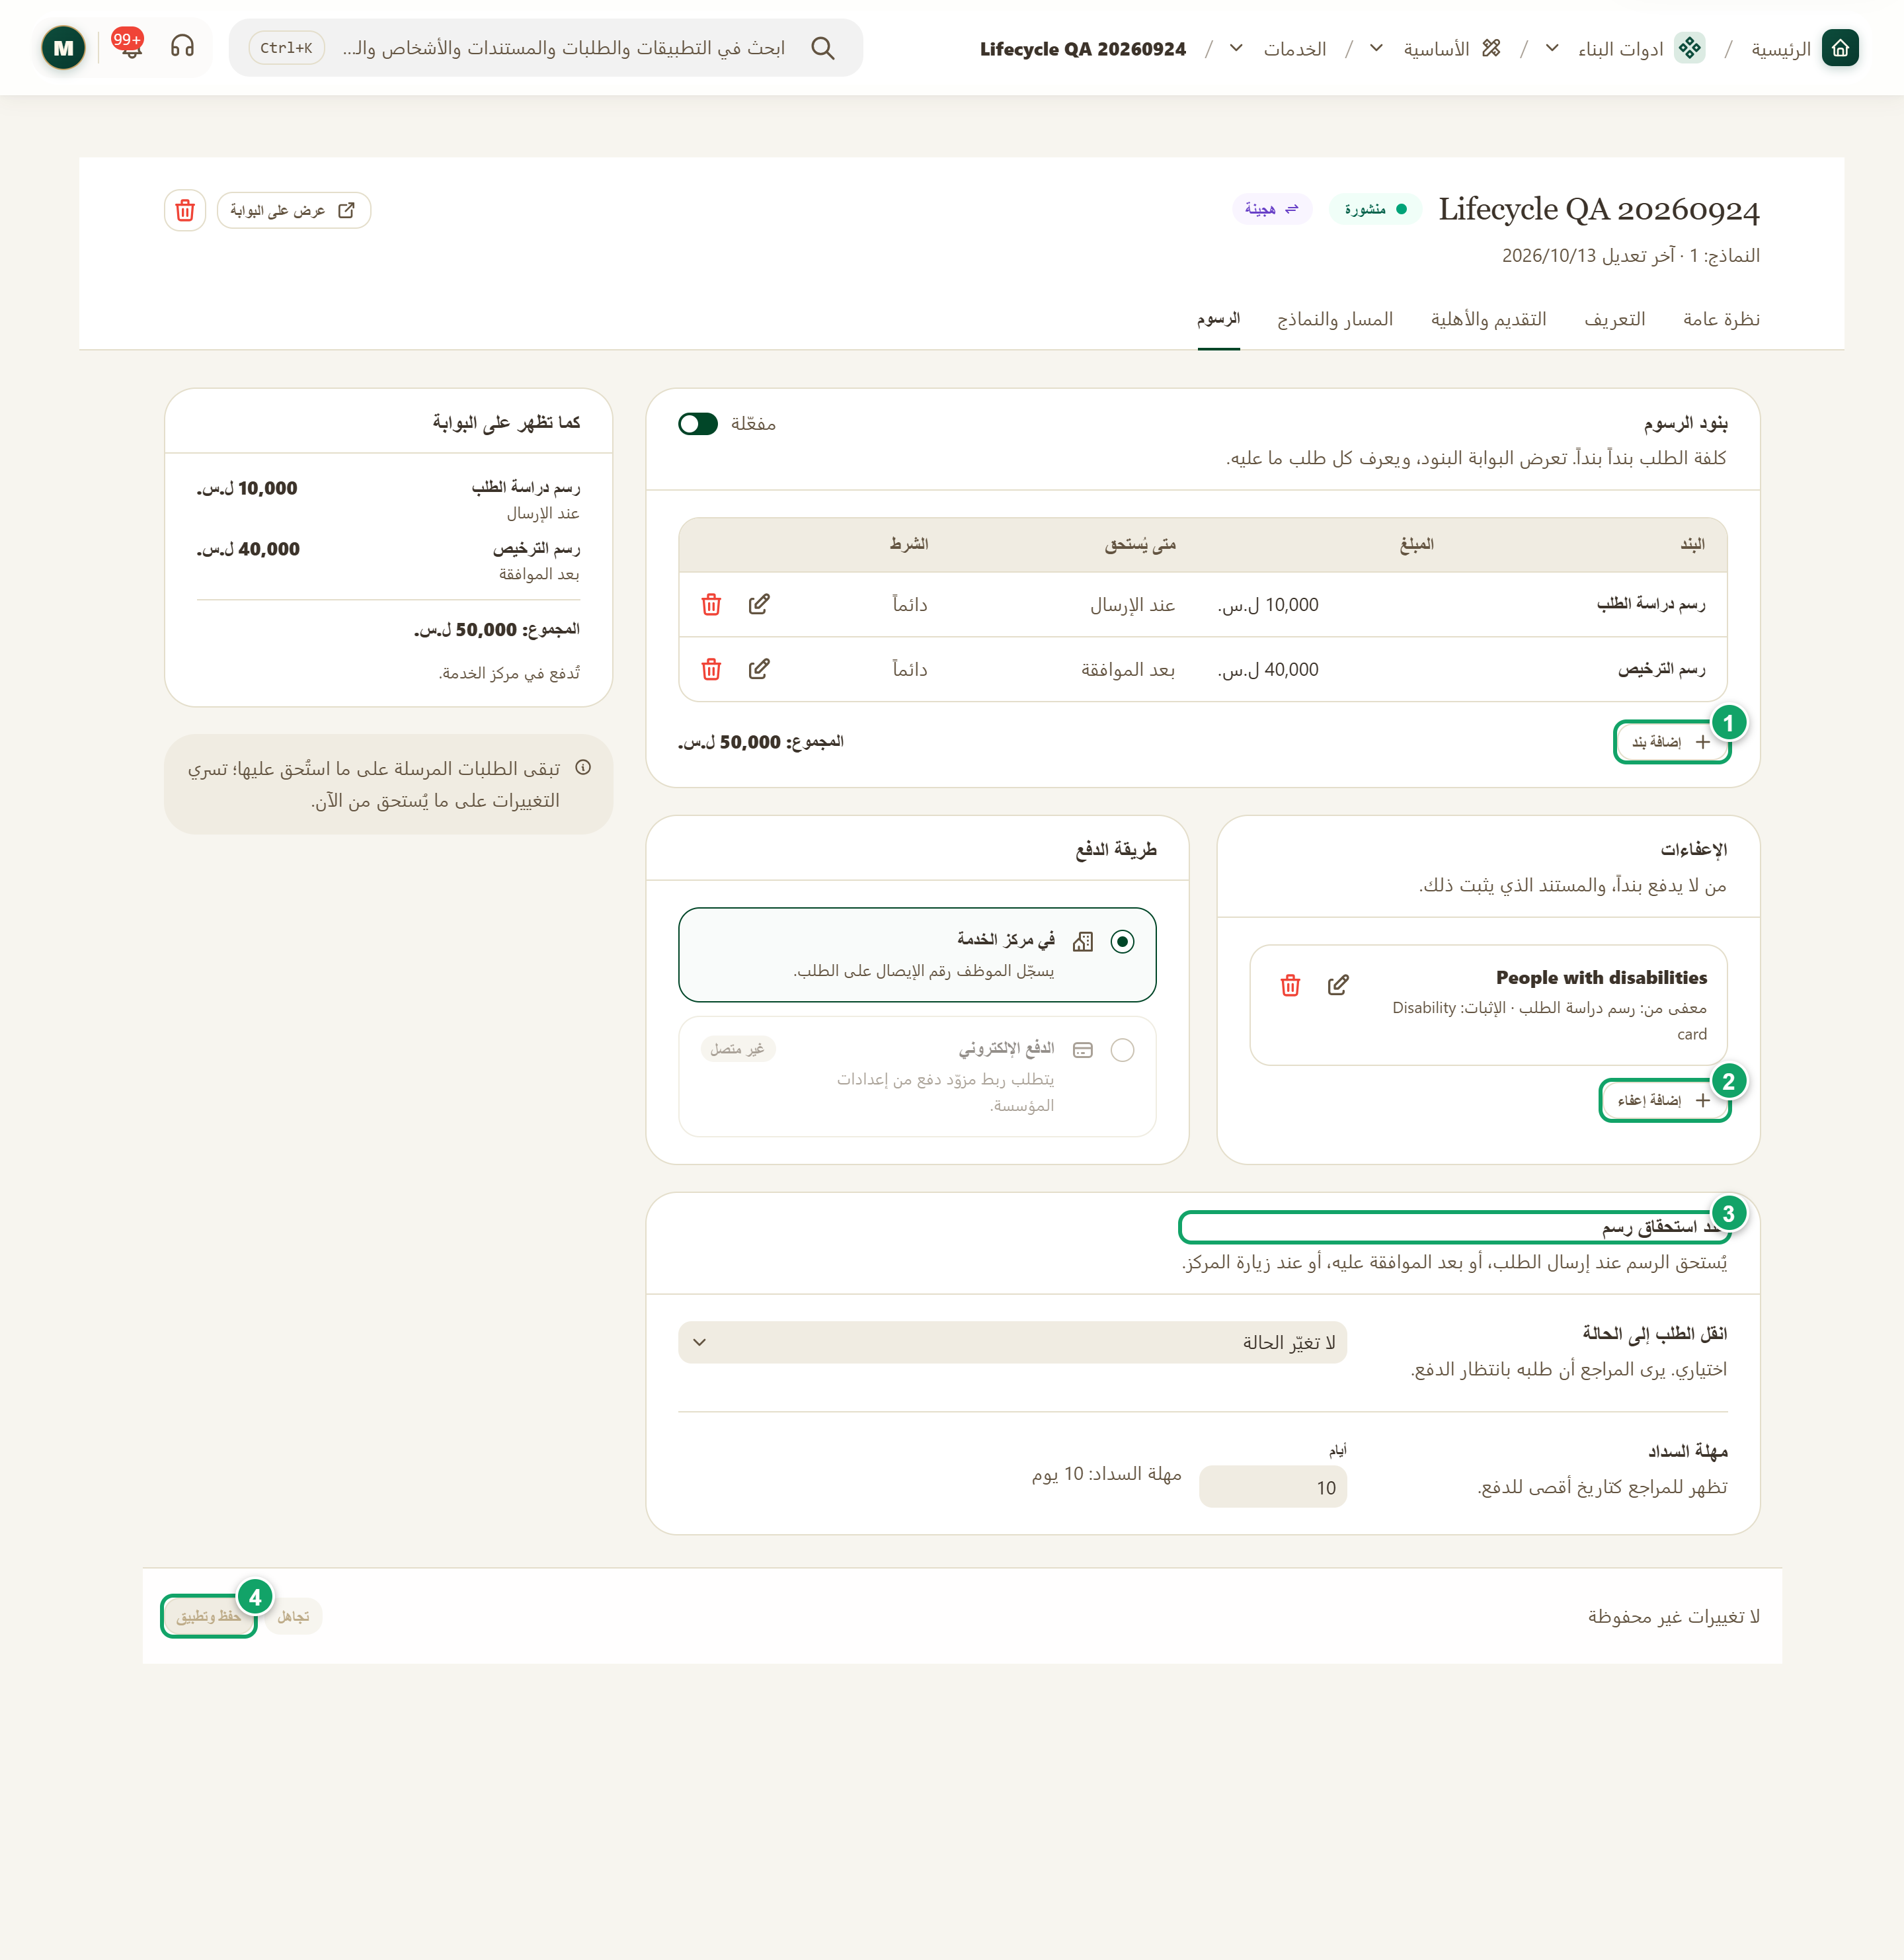
\includegraphics[width=0.95\linewidth,height=0.72\textheight,keepaspectratio]{figures/screens/ch06-services-fees-ar.png}
\caption{تبويب «الرسوم»}
\label{fig:builder-services-fees-screen}
\shotnote{تعرض الصورة رسوم خدمة في مؤسسة الاختبار: بندان بمبلغيهما ووقت استحقاق كل منهما، وإعفاء واحد، والدفع في مركز الخدمة لأن الدفع الإلكتروني «غير متصل». وتوضح المعاينة الجانبية المجموع كما يراه المتعامل، فتراجع أثر كل تغيير قبل حفظه. ① «إضافة بند». ② «إضافة إعفاء»: يضيف فئة معفاة من بند موجود. ③ «عند استحقاق رسم»: الحالة التي ينتقل إليها الطلب ومهلة السداد. ④ «حفظ وتطبيق»: يحفظ الرسوم وتسري على ما يُستحق من الآن.}
\end{figure}

\begin{table}[H]
\centering
\caption{أعمدة «بنود الرسوم»}
\label{tab:builder-services-fees-items}
\begin{tabularx}{\linewidth}{R{3.6cm} Y}
\rcHeaderRow
\thh{العمود} & \thh{ما يعنيه}\\
البند & اسم الرسم، مثل «رسم الترخيص»، وهو مطلوب.\\
المبلغ & قيمة البند بعملة الخدمة، وهو مطلوب.\\
متى يُستحق & «عند الإرسال» أو «بعد الموافقة» أو «عند زيارة المركز».\\
الشرط & «دائماً»، أو شرط يطبّق البند مع إجابات معينة في حقل اختيار من النموذج، وتختارها في «الإجابات التي يُطبَّق معها البند».\\
\end{tabularx}
\end{table}

\begin{table}[H]
\centering
\caption{بقية أقسام «الرسوم»}
\label{tab:builder-services-fees-more}
\begin{tabularx}{\linewidth}{R{3.6cm} Y}
\rcHeaderRow
\thh{القسم} & \thh{ما يقدمه}\\
الإعفاءات & «المعفَون» و«معفى من» و«الإثبات»، وخيار «يوافق الموظف على الإعفاء» إذا كان المراجِع يمنحه بعد التحقق من المستند.\\
طريقة الدفع & «في مركز الخدمة» حيث يسجّل الموظف رقم الإيصال على الطلب. أما «الدفع الإلكتروني» فيظهر «غير متصل» حتى يُربط مزوّد دفع.\\
عند استحقاق رسم & «انقل الطلب إلى الحالة» ليرى المراجع أن طلبه بانتظار الدفع، و«مهلة السداد» بالأيام.\\
كما تظهر على البوابة & معاينة البنود والمجموع كما يراها المتعامل.\\
\end{tabularx}
\end{table}

\begin{figure}[H]
\centering
\begin{tikzpicture}[node distance=0.5cm]
\node[stepBox] (a) {\RL{استخدام بنود الرسوم}};
\node[stepBox,below=of a] (b) {\RL{إضافة البنود}};
\node[stepBox,below=of b] (c) {\RL{الإعفاءات}};
\node[stepBox,below=of c] (d) {\RL{عند استحقاق رسم}};
\node[stepBox,below=of d] (e) {\RL{حفظ وتطبيق}};
\draw[flowsTo] (a) -- (b);
\draw[flowsTo] (b) -- (c);
\draw[flowsTo] (c) -- (d);
\draw[flowsTo] (d) -- (e);
\end{tikzpicture}
\rclegend
\caption{إعداد رسوم الخدمة}
\label{fig:builder-services-fees-flow}
\shotnote{تأتي البنود قبل الإعفاءات لأن الإعفاء يشير إلى بنود موجودة، ولا يمكن إضافته قبلها. وتبقى الطلبات المرسلة على ما استُحق عليها، أما التغييرات فتسري على ما يُستحق من الآن.}
\end{figure}

\subsection{خطوات العمل والتحقق}
\begin{enumerate}
\item افتح الخدمة واضغط «الرسوم»، ثم فعّل «استخدام بنود الرسوم».
\item اضغط «إضافة بند»، واكتب «اسم البند» والمبلغ، واختر متى يُستحق وشرطه، ثم اضغط «تم».
\item أضف الإعفاءات بزر «إضافة إعفاء» إن وُجدت.
\item اختر في «عند استحقاق رسم» الحالة التي ينتقل إليها الطلب و«مهلة السداد».
\item اضغط «حفظ وتطبيق»، وراجع المجموع في «كما تظهر على البوابة».
\end{enumerate}

\textbf{تحقق ومعالجة المشكلة:} يظهر عدد البنود في بند «الرسوم» من «جاهزية الخدمة». فإذا بقي الحفظ معطلاً، فاقرأ «يحتاج كل بند إلى اسم ومبلغ.» وأكمل البند الناقص. وإذا عُطّل «إضافة إعفاء»، فأضف بنداً واحداً على الأقل أولاً.

\clearpage
\section{إتاحة نموذج على البوابة}
\label{sec:builder-feature-services-publish}

قد يكون لديك نموذج داخلي منشور تريد أن يصل إلى المتعاملين. فبدلاً من إنشاء خدمة من الصفر، يحوّله زر «إتاحته على البوابة» في خطوة واحدة إلى خدمة جديدة، أو يضيفه خطوةً إلى خدمة قائمة. وتبدأ الخدمة الجديدة بإعدادات المؤسسة الافتراضية، ثم تغيّرها من صفحة الخدمة متى شئت دون إعادة نشر النموذج.

\textbf{المسار ومن يستخدمه:} «الخدمات» ← «نماذج داخلية» ← «إتاحته على البوابة»، أو من تبويب «الخدمة» في إعدادات النموذج. يستخدمه مسؤول الخدمات عندما يصبح نموذج داخلي خدمةً للجمهور.

\begin{rcnote}[مثال: شركة الأفق]
تملك الأفق نموذجاً داخلياً منشوراً لتجديد طلب الزيارة، فيضغط مسؤول النظام «إتاحته على البوابة» ويختار «خطوة في خدمة قائمة». ثم يختار خدمة «طلب زيارة فرع» ويضيفه بصفة «نموذج خارج المسار»، فيبدؤه العميل في أي وقت.
\end{rcnote}

\begin{table}[H]
\centering
\caption{خيارات نافذة الإتاحة}
\label{tab:builder-services-publish-options}
\begin{tabularx}{\linewidth}{R{3.6cm} Y}
\rcHeaderRow
\thh{الخيار} & \thh{ما يعنيه}\\
خدمة جديدة & الحالة الأبسط: خدمة واحدة لهذا النموذج. وتكتب «اسم الخدمة على البوابة».\\
من يعبّئ هذا النموذج & «المتعامل عبر البوابة» فتُنشأ الخدمة «إلكترونية بالكامل»، أو «الموظف في المركز» فتُنشأ «تقليدية مع تتبّع إلكتروني».\\
انشر الخدمة على البوابة الآن & عند تحديده يصبح الزر «إنشاء الخدمة ونشرها»، وعند إلغائه يصبح «إنشاء الخدمة كمسودة».\\
خطوة في خدمة قائمة & تختار «الخدمة» من الخدمات التي تبدأ إلكترونياً، ثم «يُضاف كـ»: «نموذج خارج المسار» أو «خطوة في المسار»، وتضغط «إضافة إلى الخدمة».\\
\end{tabularx}
\end{table}

وتظهر في الخدمة الجديدة إعدادات افتراضية: يقدّم أي شخص، بدون مستوى تحقق، مفتوحة دائماً، بلا حدود. أما النموذج المضاف إلى خدمة قائمة فيتبع أهليتها ومستوى التحقق فيها. وتجد في قائمة الخدمات أحياناً نموذجاً بشارة «من إعدادات النموذج»، وهو منشور للعامة بإعداداته القديمة؛ فاضغط «إنشاء خدمة» لتديره كبقية الخدمات.

\begin{figure}[H]
\centering
\begin{tikzpicture}[node distance=0.5cm]
\node[stepBox] (a) {\RL{نشر النموذج في المنشئ}};
\node[stepBox,below=of a] (b) {\RL{إتاحته على البوابة}};
\node[stepBox,below=of b] (c) {\RL{خدمة جديدة أو قائمة}};
\node[stepBox,below=of c] (d) {\RL{الإنشاء أو الإضافة}};
\node[stepBox,below=of d] (e) {\RL{مراجعة صفحة الخدمة}};
\draw[flowsTo] (a) -- (b);
\draw[flowsTo] (b) -- (c);
\draw[flowsTo] (c) -- (d);
\draw[flowsTo] (d) -- (e);
\end{tikzpicture}
\rclegend
\caption{تحويل نموذج داخلي إلى خدمة}
\label{fig:builder-services-publish-flow}
\shotnote{يبدأ المخطط بنشر النموذج لأن زر الإتاحة يبقى معطلاً حتى ذلك الحين. وينتهي بصفحة الخدمة لأن الإعدادات الافتراضية تناسب البداية فقط، فراجع الأهلية والدليل قبل أن تعتمد الخدمة.}
\end{figure}

\subsection{خطوات العمل والتحقق}
\begin{enumerate}
\item افتح «الخدمات» وابحث عن النموذج في «نماذج داخلية».
\item اضغط «إتاحته على البوابة»، واختر «خدمة جديدة» أو «خطوة في خدمة قائمة».
\item للخدمة الجديدة: اكتب الاسم واختر «من يعبّئ هذا النموذج»، وقرّر هل تحدد «انشر الخدمة على البوابة الآن».
\item للخدمة القائمة: اختر «الخدمة» و«يُضاف كـ»، ثم اضغط «إضافة إلى الخدمة».
\end{enumerate}

\textbf{تحقق ومعالجة المشكلة:} تُفتح صفحة الخدمة مباشرة، ويختفي النموذج من «نماذج داخلية». فإذا كان الزر معطلاً مع التلميح «انشر النموذج في المنشئ أولاً»، فانشر النموذج ثم عُد. وإذا ظهر «لا توجد خدمات تبدأ إلكترونياً بعد»، فأنشئ خدمة جديدة بدلاً من الإضافة.

\clearpage
\section{الخدمة في إعدادات النموذج}
\label{sec:builder-feature-services-form-settings}

لا تحتاج إلى مغادرة منشئ النماذج لتعرف علاقة النموذج بالخدمات. ففي إعدادات النموذج تبويب «الخدمة» يبيّن الخدمة التي ينتمي إليها النموذج ودوره فيها، وما تحدده الخدمة له، وهل يتوافق معها. ويذكّرك التبويب بقاعدة مهمة: إعدادات الخدمة تسري فوراً من صفحتها، أما تغييرات النموذج فتسري بعد نشره.

\textbf{المسار ومن يستخدمه:} «النماذج» ← افتح النموذج ← «الإعدادات» ← «الخدمة» في نافذة «إعدادات النموذج». يستخدمه من يعدّل النموذج ليتأكد من أن تعديله لا يكسر مسار الخدمة.

\begin{rcnote}[مثال: شركة الأفق]
يفتح مسؤول النظام تبويب «الخدمة» ① في نموذج «طلب زيارة فرع»، فيرى أنه «الخطوة 1 في المسار» مع شارة «نقطة البدء». ويقرأ في «توافق النموذج مع الخدمة» ④ أن الحالات التي يعتمد عليها المسار موجودة في النموذج.
\end{rcnote}

\begin{figure}[H]
\centering
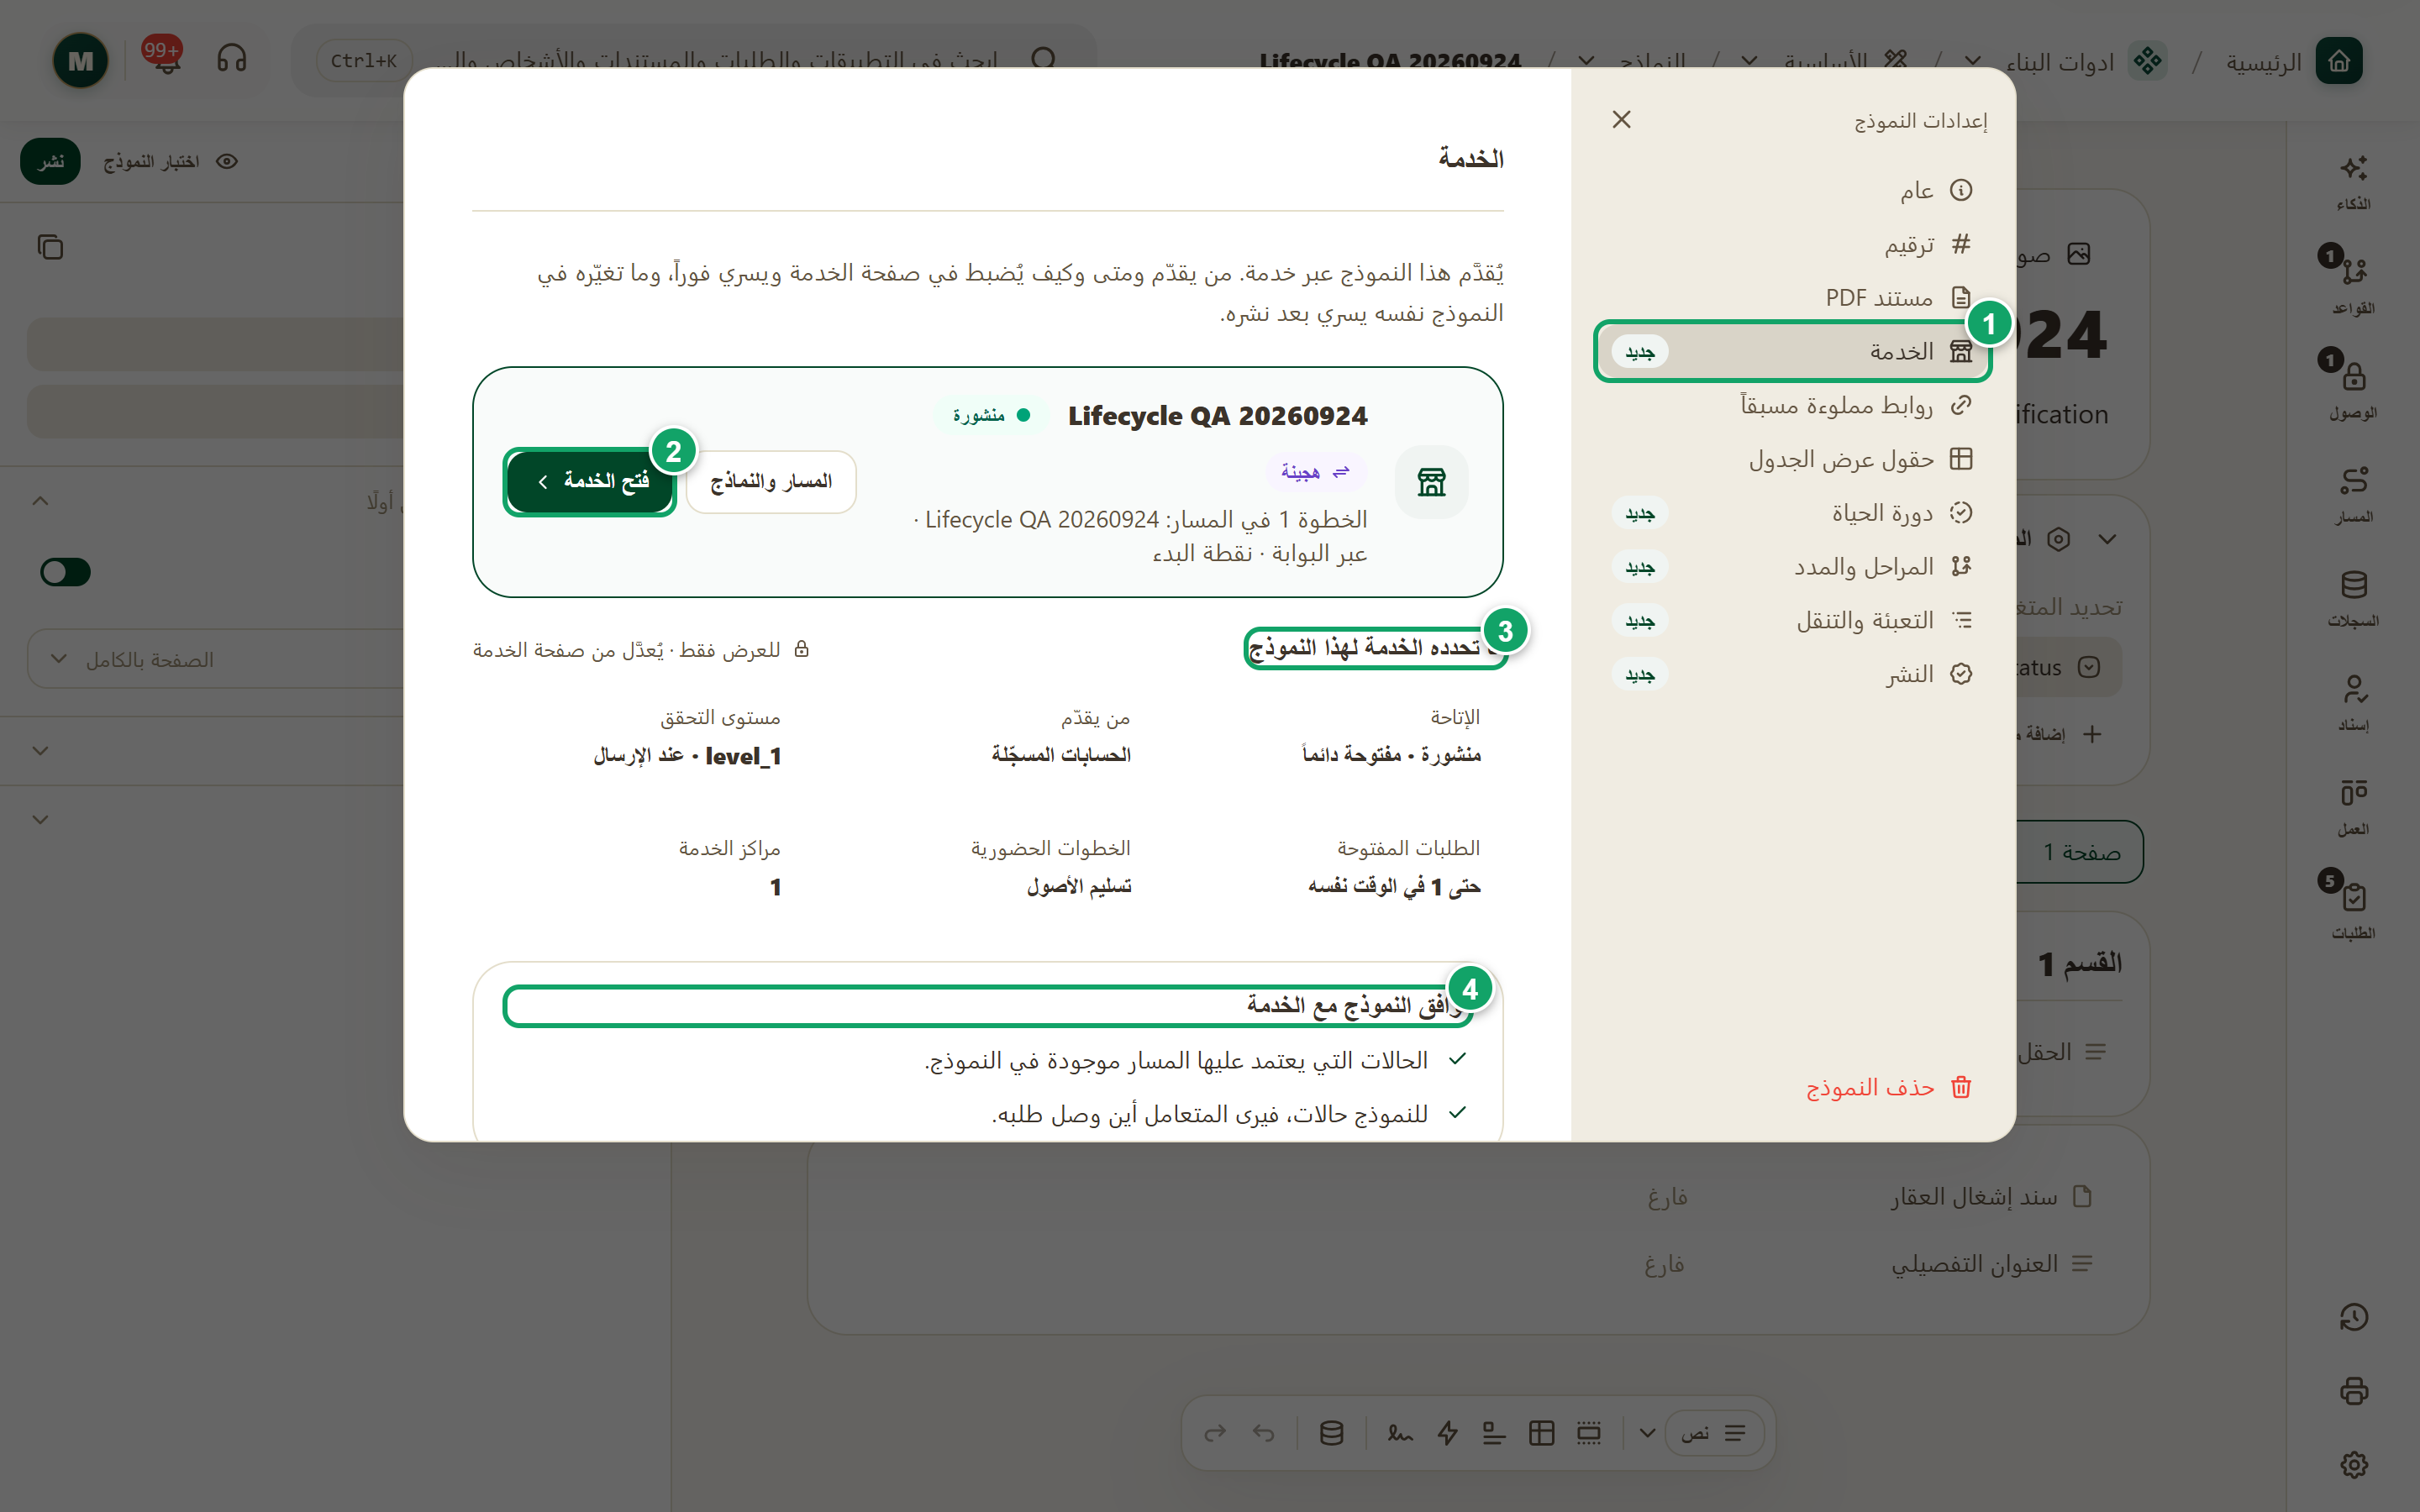
\includegraphics[width=0.95\linewidth,height=0.72\textheight,keepaspectratio]{figures/screens/ch06-services-form-settings-ar.png}
\caption{تبويب «الخدمة» في «إعدادات النموذج»}
\label{fig:builder-services-form-settings-screen}
\shotnote{تعرض الصورة تبويب «الخدمة» لنموذج البدء في خدمة هجينة بمؤسسة الاختبار، وفيه دور النموذج «الخطوة 1 في المسار» وإعدادات الخدمة التي تنطبق عليه. وتبيّن أن هذه الإعدادات «للعرض فقط»، فالتعديل يجري في صفحة الخدمة لا في منشئ النماذج. ① «الخدمة». ② «فتح الخدمة»: ينقلك إلى صفحة الخدمة لتعديلها. ③ «ما تحدده الخدمة لهذا النموذج»: الإتاحة ومن يقدّم والتحقق والحدود والمراكز. ④ «توافق النموذج مع الخدمة»: فحوص الحالات التي يعتمد عليها المسار.}
\end{figure}

\begin{table}[H]
\centering
\caption{ما يعرضه تبويب «الخدمة»}
\label{tab:builder-services-form-settings-parts}
\begin{tabularx}{\linewidth}{R{3.6cm} Y}
\rcHeaderRow
\thh{الجزء} & \thh{ما يعرضه أو يتيحه}\\
الخدمة ودور النموذج & اسم الخدمة ودور النموذج، مثل «الخطوة 1 في المسار» أو «نموذج خارج المسار، متاح في أي وقت»، مع رابطي «المسار والنماذج» و«فتح الخدمة».\\
ما تحدده الخدمة لهذا النموذج & «الإتاحة» و«من يقدّم» و«مستوى التحقق» و«الطلبات المفتوحة» و«الخطوات الحضورية» و«مراكز الخدمة»، وهي «للعرض فقط · يُعدَّل من صفحة الخدمة».\\
توافق النموذج مع الخدمة & يتحقق من وجود الحالات التي ينتظرها المسار في النموذج، ومن أن للنموذج حالات يرى بها المتعامل أين وصل طلبه.\\
إزالته من الخدمة & يجعل النموذج داخلياً ويخفيه من البوابة. ويُعطَّل لنموذج البدء في الخدمات التي تبدأ عبر البوابة حتى تعدّل المسار.\\
نموذج داخلي & للنموذج الذي لا ينتمي إلى خدمة، ومعه زر «إتاحته على البوابة».\\
معالجة الطلبات & مفتاح «مساحة المراجعة وتحديثات مقدمي الطلبات» لهذا النموذج، ومفتاح «إغلاق الطلب من المراسلات».\\
\end{tabularx}
\end{table}

\begin{figure}[H]
\centering
\begin{tikzpicture}[node distance=0.5cm]
\node[stepBox] (a) {\RL{فتح تبويب الخدمة}};
\node[stepBox,below=of a] (b) {\RL{قراءة دور النموذج}};
\node[stepBox,below=of b] (c) {\RL{مراجعة التوافق}};
\node[stepBox,below=of c] (d) {\RL{الإصلاح في النموذج أو الخدمة}};
\draw[flowsTo] (a) -- (b);
\draw[flowsTo] (b) -- (c);
\draw[flowsTo] (c) -- (d);
\end{tikzpicture}
\rclegend
\caption{فحص علاقة النموذج بخدمته}
\label{fig:builder-services-form-settings-flow}
\shotnote{يضع المخطط مراجعة التوافق قبل أي إصلاح، لأن التحذير يحدد مكان الحل: إما حالات النموذج في «دورة الحياة»، وإما خطوات الخدمة في «المسار والنماذج». ولا تُعدَّل إعدادات الخدمة من هذا التبويب، فهو للعرض فقط.}
\end{figure}

\subsection{خطوات العمل والتحقق}
\begin{enumerate}
\item افتح النموذج في منشئ النماذج، واضغط «الإعدادات» ثم «الخدمة».
\item اقرأ دور النموذج في الخدمة وما تحدده له.
\item راجع «توافق النموذج مع الخدمة»، وأصلح أي تحذير في «دورة الحياة» أو في «المسار والنماذج».
\item إذا لم ينتمِ النموذج إلى خدمة، فاضغط «إتاحته على البوابة» لتحويله إلى خدمة.
\end{enumerate}

\textbf{تحقق ومعالجة المشكلة:} يجب أن تظهر علامة صح بجانب كل فحص في «توافق النموذج مع الخدمة». فإذا ظهر «احفظ النموذج أولاً.»، فاحفظ النموذج الجديد ثم افتح التبويب من جديد. وإذا كان «إزالته من الخدمة» معطلاً، فغيّر نموذج البدء في «المسار والنماذج» أولاً.

\clearpage
\section{مكتب الاستقبال}
\label{sec:builder-feature-services-intake}

مكتب الاستقبال هو الصفحة التي يسجّل فيها موظف المركز طلب متعامل حضر بنفسه. فيختار الخدمة، ويبحث عن حساب المتعامل أو يسجّله دونه، ويؤشّر المستندات التي استلمها، ثم يعبّئ النموذج معه ويطبع إيصالاً برقم الطلب. وبذلك يدخل الطلب الحضوري في المتابعة نفسها التي تمر بها طلبات البوابة.

\textbf{المسار ومن يستخدمه:} «الخدمات» ← «مكتب الاستقبال». يستخدمه موظفو مراكز الخدمة يومياً، ويظهر فيه فقط ما فعّل «الاستقبال في المركز» من الخدمات.

\begin{rcnote}[مثال: شركة الأفق]
يحضر عميل إلى فرع حلب بلا حساب على البوابة، فيضغط عمر حداد «طلب حضوري جديد» ② ويختار «تسجيل مراجع بلا حساب»، ويكتب اسمه ورقم هاتفه. ثم يعبّئ النموذج معه ويضغط «تسجيل وطباعة الإيصال».
\end{rcnote}

\begin{figure}[H]
\centering
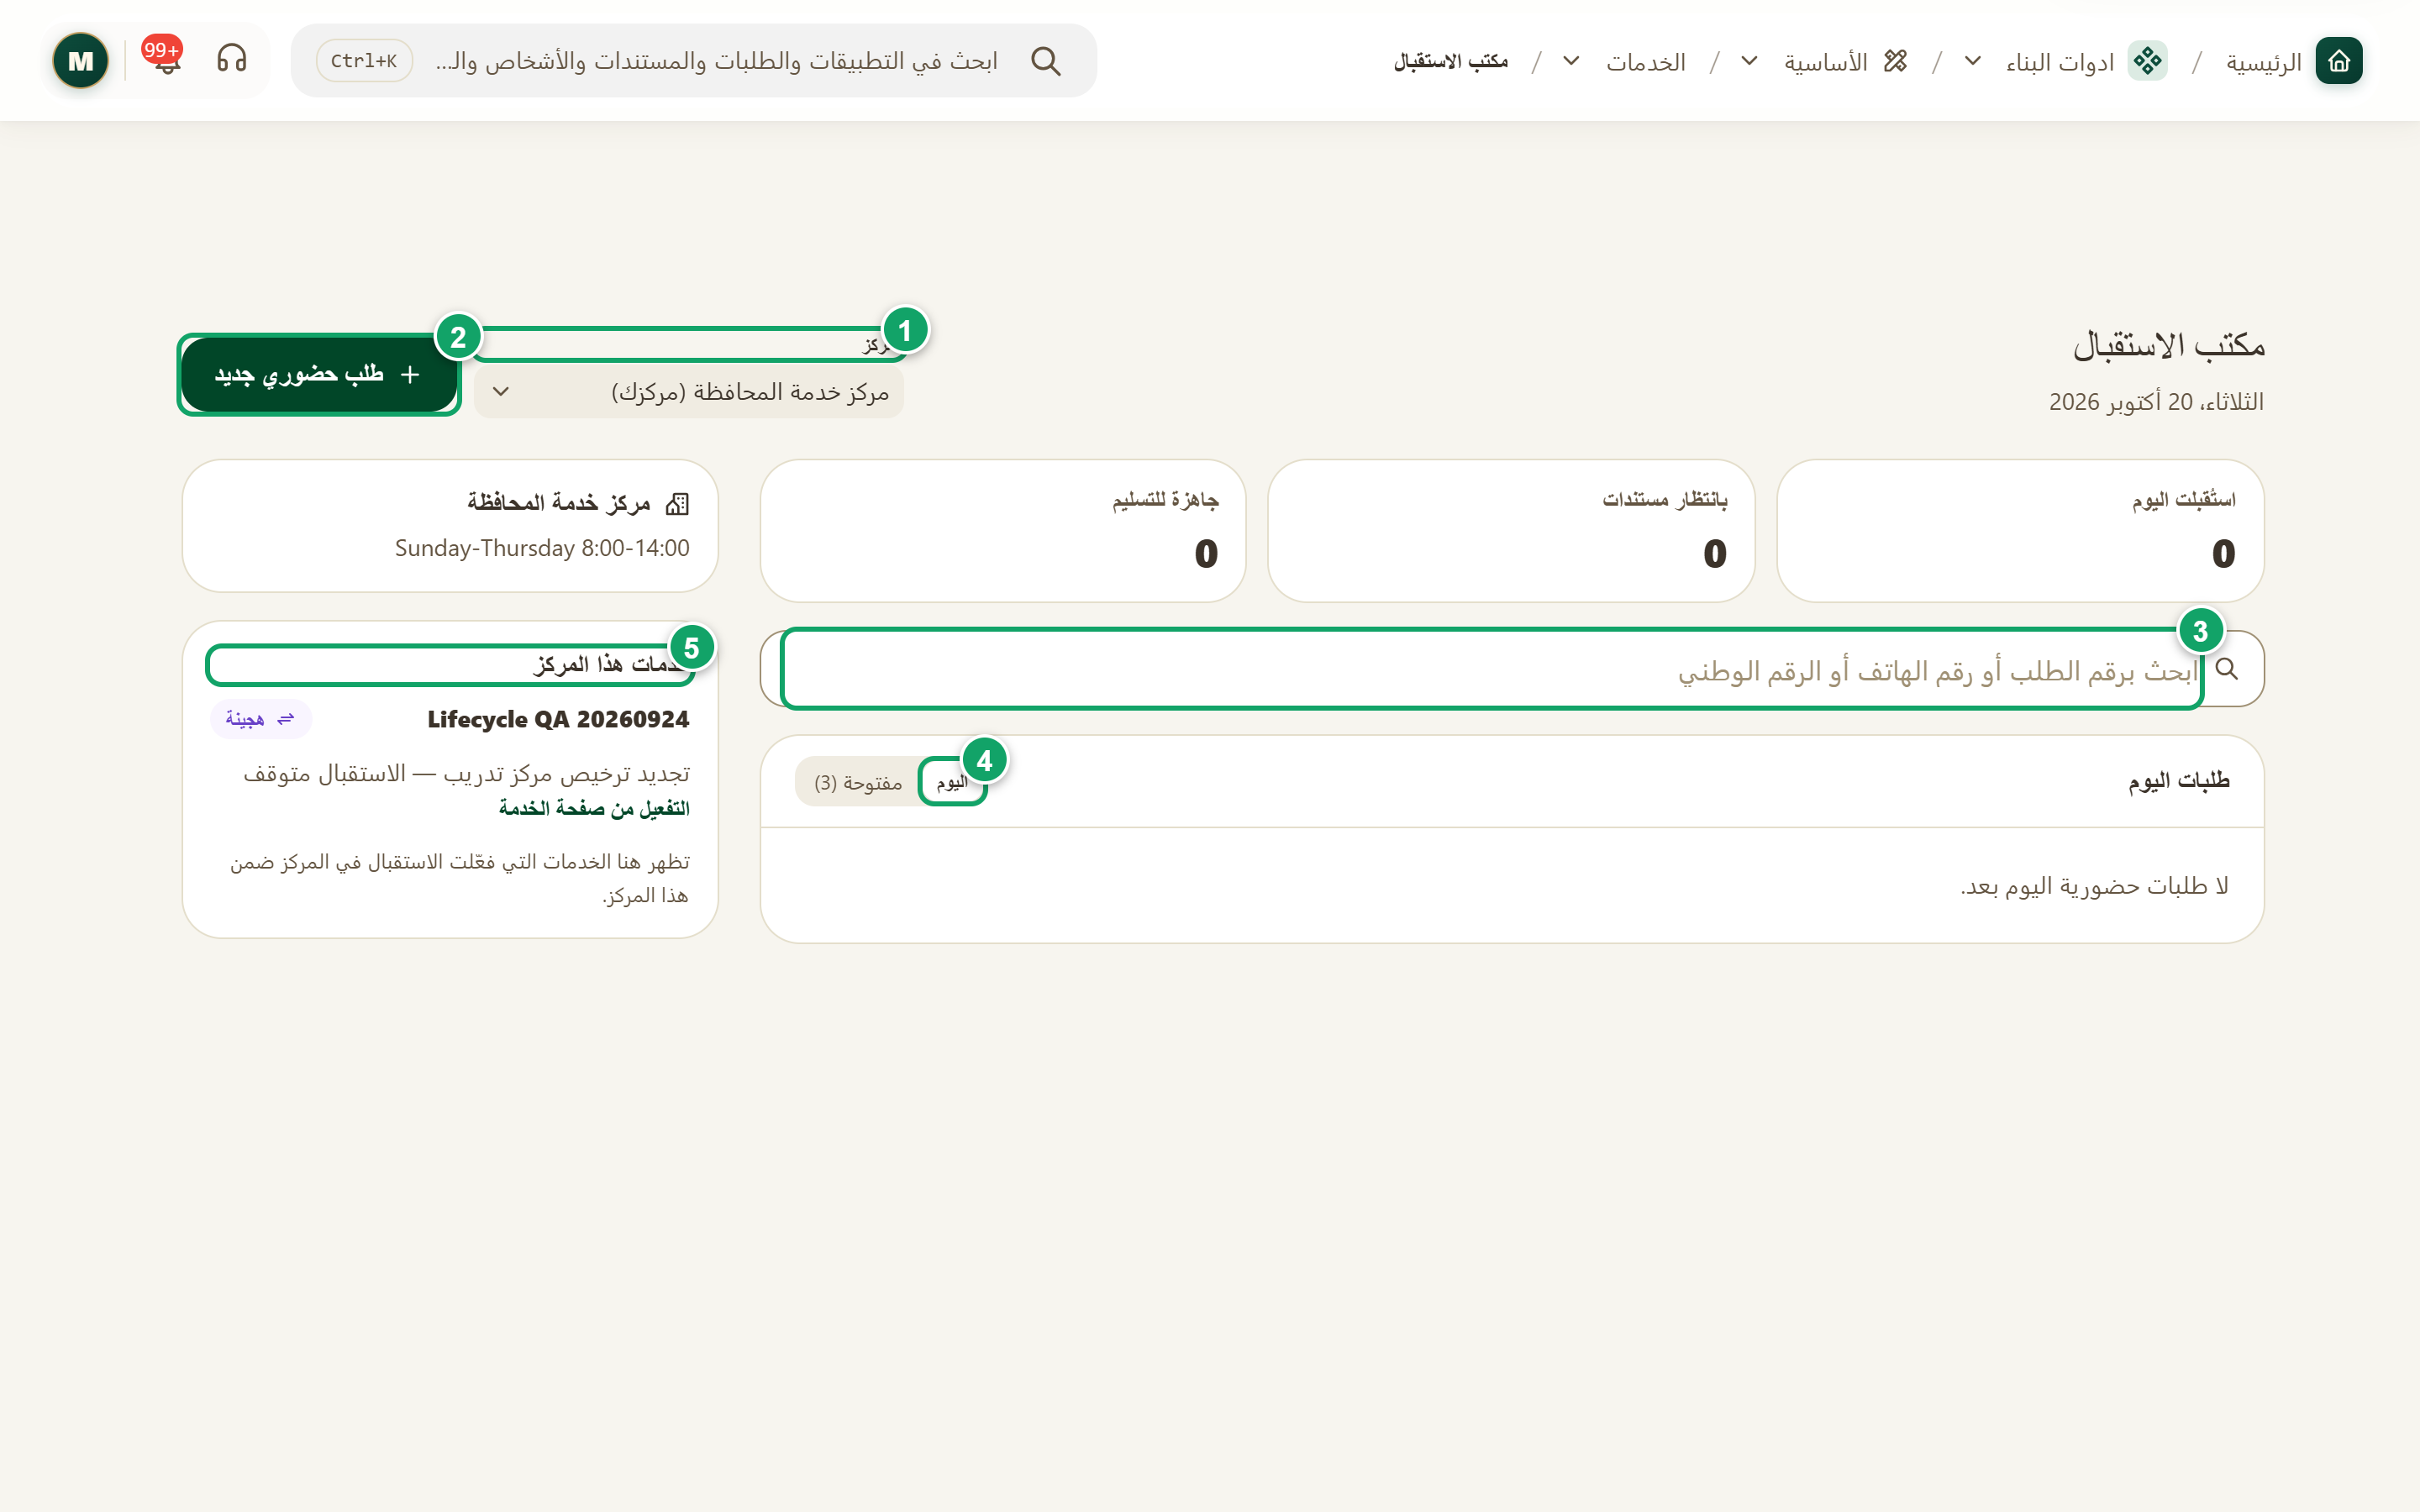
\includegraphics[width=0.95\linewidth,height=0.72\textheight,keepaspectratio]{figures/screens/ch06-services-intake-ar.png}
\caption{صفحة «مكتب الاستقبال»}
\label{fig:builder-services-intake-screen}
\shotnote{تعرض الصورة مكتب الاستقبال في مؤسسة الاختبار على «مركز خدمة المحافظة»، ولم يُسجَّل فيه طلب حضوري اليوم، لذلك تظهر المؤشرات أصفاراً. وتبيّن قائمة خدمات المركز أن خدمة واحدة تستقبل الطلبات، وأن أخرى متوقفة مع رابط لتفعيلها. ① «المركز». ② «طلب حضوري جديد»: يبدأ تسجيل طلب لمتعامل حاضر. ③ مربع البحث: يبحث برقم الطلب أو رقم الهاتف أو الرقم الوطني. ④ «اليوم»: يعرض طلبات اليوم، وبجانبه «مفتوحة». ⑤ «خدمات هذا المركز»: الخدمات التي فعّلت الاستقبال.}
\end{figure}

\begin{table}[H]
\centering
\caption{أجزاء مكتب الاستقبال}
\label{tab:builder-services-intake-desk}
\begin{tabularx}{\linewidth}{R{3.6cm} Y}
\rcHeaderRow
\thh{الجزء} & \thh{ما يعرضه أو يتيحه}\\
المركز & المركز الذي تعمل عليه، ويُعلَّم مركزك بعبارة «(مركزك)».\\
المؤشرات & «استُقبلت اليوم» أو «مفتوحة في هذا المركز»، و«بانتظار مستندات»، و«جاهزة للتسليم».\\
البحث والعرض & «ابحث برقم الطلب أو رقم الهاتف أو الرقم الوطني»، والتبديل بين «اليوم» و«مفتوحة».\\
جدول الطلبات & «رقم الطلب» و«المراجع» و«الخدمة» و«الحالة» و«استلمه» و«الوقت»، مع «عرض» أو «متابعة» و«طباعة الإيصال».\\
خدمات هذا المركز & الخدمات التي فعّلت الاستقبال، ورابط «التفعيل من صفحة الخدمة» لما توقف منها.\\
\end{tabularx}
\end{table}

\begin{table}[H]
\centering
\caption{صفحة «طلب حضوري جديد» والإيصال}
\label{tab:builder-services-intake-new}
\begin{tabularx}{\linewidth}{R{3.6cm} Y}
\rcHeaderRow
\thh{القسم} & \thh{ما تفعله فيه}\\
الخدمة والمراجع & تختار الخدمة، ثم تبحث بـ«رقم الهاتف أو البريد أو الرقم الوطني» عن حساب المراجع ليظهر الطلب في حسابه، أو تختار «تسجيل مراجع بلا حساب» وتكتب «الاسم الكامل» و«رقم الهاتف».\\
المستندات المستلمة & قائمة المستندات من دليل الخدمة. وإذا نقص مستند «مطلوب» يبقى الطلب «بانتظار مستندات».\\
ملخص & الحالة «عند التسجيل»، والرسم المستلم في المركز مع «رقم الإيصال»، ثم زر «إنشاء وتعبئة البيانات».\\
إيصال استلام طلب & يحمل «رقم الطلب» والمستندات المستلمة وغير المستلمة، وطريقة «تتبّع طلبك» برقم الطلب ورقم الهاتف، ودوام المركز.\\
\end{tabularx}
\end{table}

\begin{figure}[H]
\centering
\begin{tikzpicture}[node distance=0.5cm]
\node[stepBox] (a) {\RL{طلب حضوري جديد}};
\node[stepBox,below=of a] (b) {\RL{الخدمة والمراجع}};
\node[stepBox,below=of b] (c) {\RL{المستندات المستلمة}};
\node[stepBox,below=of c] (d) {\RL{إنشاء وتعبئة البيانات}};
\node[stepBox,below=of d] (e) {\RL{تسجيل وطباعة الإيصال}};
\draw[flowsTo] (a) -- (b);
\draw[flowsTo] (b) -- (c);
\draw[flowsTo] (c) -- (d);
\draw[flowsTo] (d) -- (e);
\end{tikzpicture}
\rclegend
\caption{تسجيل طلب حضوري}
\label{fig:builder-services-intake-flow}
\shotnote{يُنشأ الطلب أولاً ثم يُعبَّأ نموذجه، ولا يأخذ رقمه إلا عند الخطوة الأخيرة، لذلك يظهر في الجدول بعبارة «غير مسجّل» حتى تُكمله. وإذا نقص مستند مطلوب، يبقى الطلب بانتظاره حتى تضغط «استُلمت المستندات — إرسال الطلب».}
\end{figure}

\subsection{خطوات العمل والتحقق}
\begin{enumerate}
\item افتح «الخدمات» واضغط «مكتب الاستقبال»، وتأكد من «المركز».
\item اضغط «طلب حضوري جديد»، واختر الخدمة، ثم ابحث عن المراجع أو سجّله بلا حساب.
\item أشّر المستندات المستلمة، وسجّل «رقم الإيصال» إن استلمت الرسم، ثم اضغط «إنشاء وتعبئة البيانات».
\item عبّئ النموذج مع المراجع، ثم اضغط «تسجيل وطباعة الإيصال».
\item اضغط «طباعة» في صفحة الإيصال وسلّمه للمراجع.
\end{enumerate}

\textbf{تحقق ومعالجة المشكلة:} يظهر الطلب في الجدول برقمه واسم من استلمه. فإذا ظهر «أكمل الإجابات المطلوبة في النموذج قبل تسجيل الطلب.»، فأكمل الحقول الناقصة. وإذا ظهر «لا تستقبل أي خدمة طلبات حضورية في هذا المركز بعد»، ففعّل «الاستقبال في المركز» في تبويب «التقديم والأهلية» للخدمة.

\clearpage
\section{أداء الخدمات}
\label{sec:builder-feature-services-performance}

تجيب صفحة «أداء الخدمات» عن أسئلة الإدارة: كم طلباً وصل، وكم استغرق إنجازه، وأين يتأخر، وما رأي المتعاملين. وتُحتسب فيها الطلبات المرسلة من البوابة، ولا يدخل وقت انتظار المتعامل في مدد المراحل والإنجاز. لذلك تعطيك صورة عادلة عن أداء فريقك، وتدلك على المرحلة التي تحتاج إلى دعم.

\textbf{المسار ومن يستخدمه:} «الخدمات» ← «أداء الخدمات»، أو رابط «الأداء الكامل» في «نظرة عامة». يستخدمها مديرو الخدمات في مراجعتهم الدورية.

\begin{rcnote}[مثال: شركة الأفق]
تختار سارة الخطيب «آخر 30 يوم» ① وخدمة «طلب زيارة فرع»، فترى في «طلبات تجاوزت المدة» ③ طلباً متأخراً في مرحلة المراجعة. فتضغط «تصعيد» بجانبه، ثم تصدّر المؤشرات بزر «تصدير» ④ لاجتماعها الشهري.
\end{rcnote}

\begin{figure}[H]
\centering
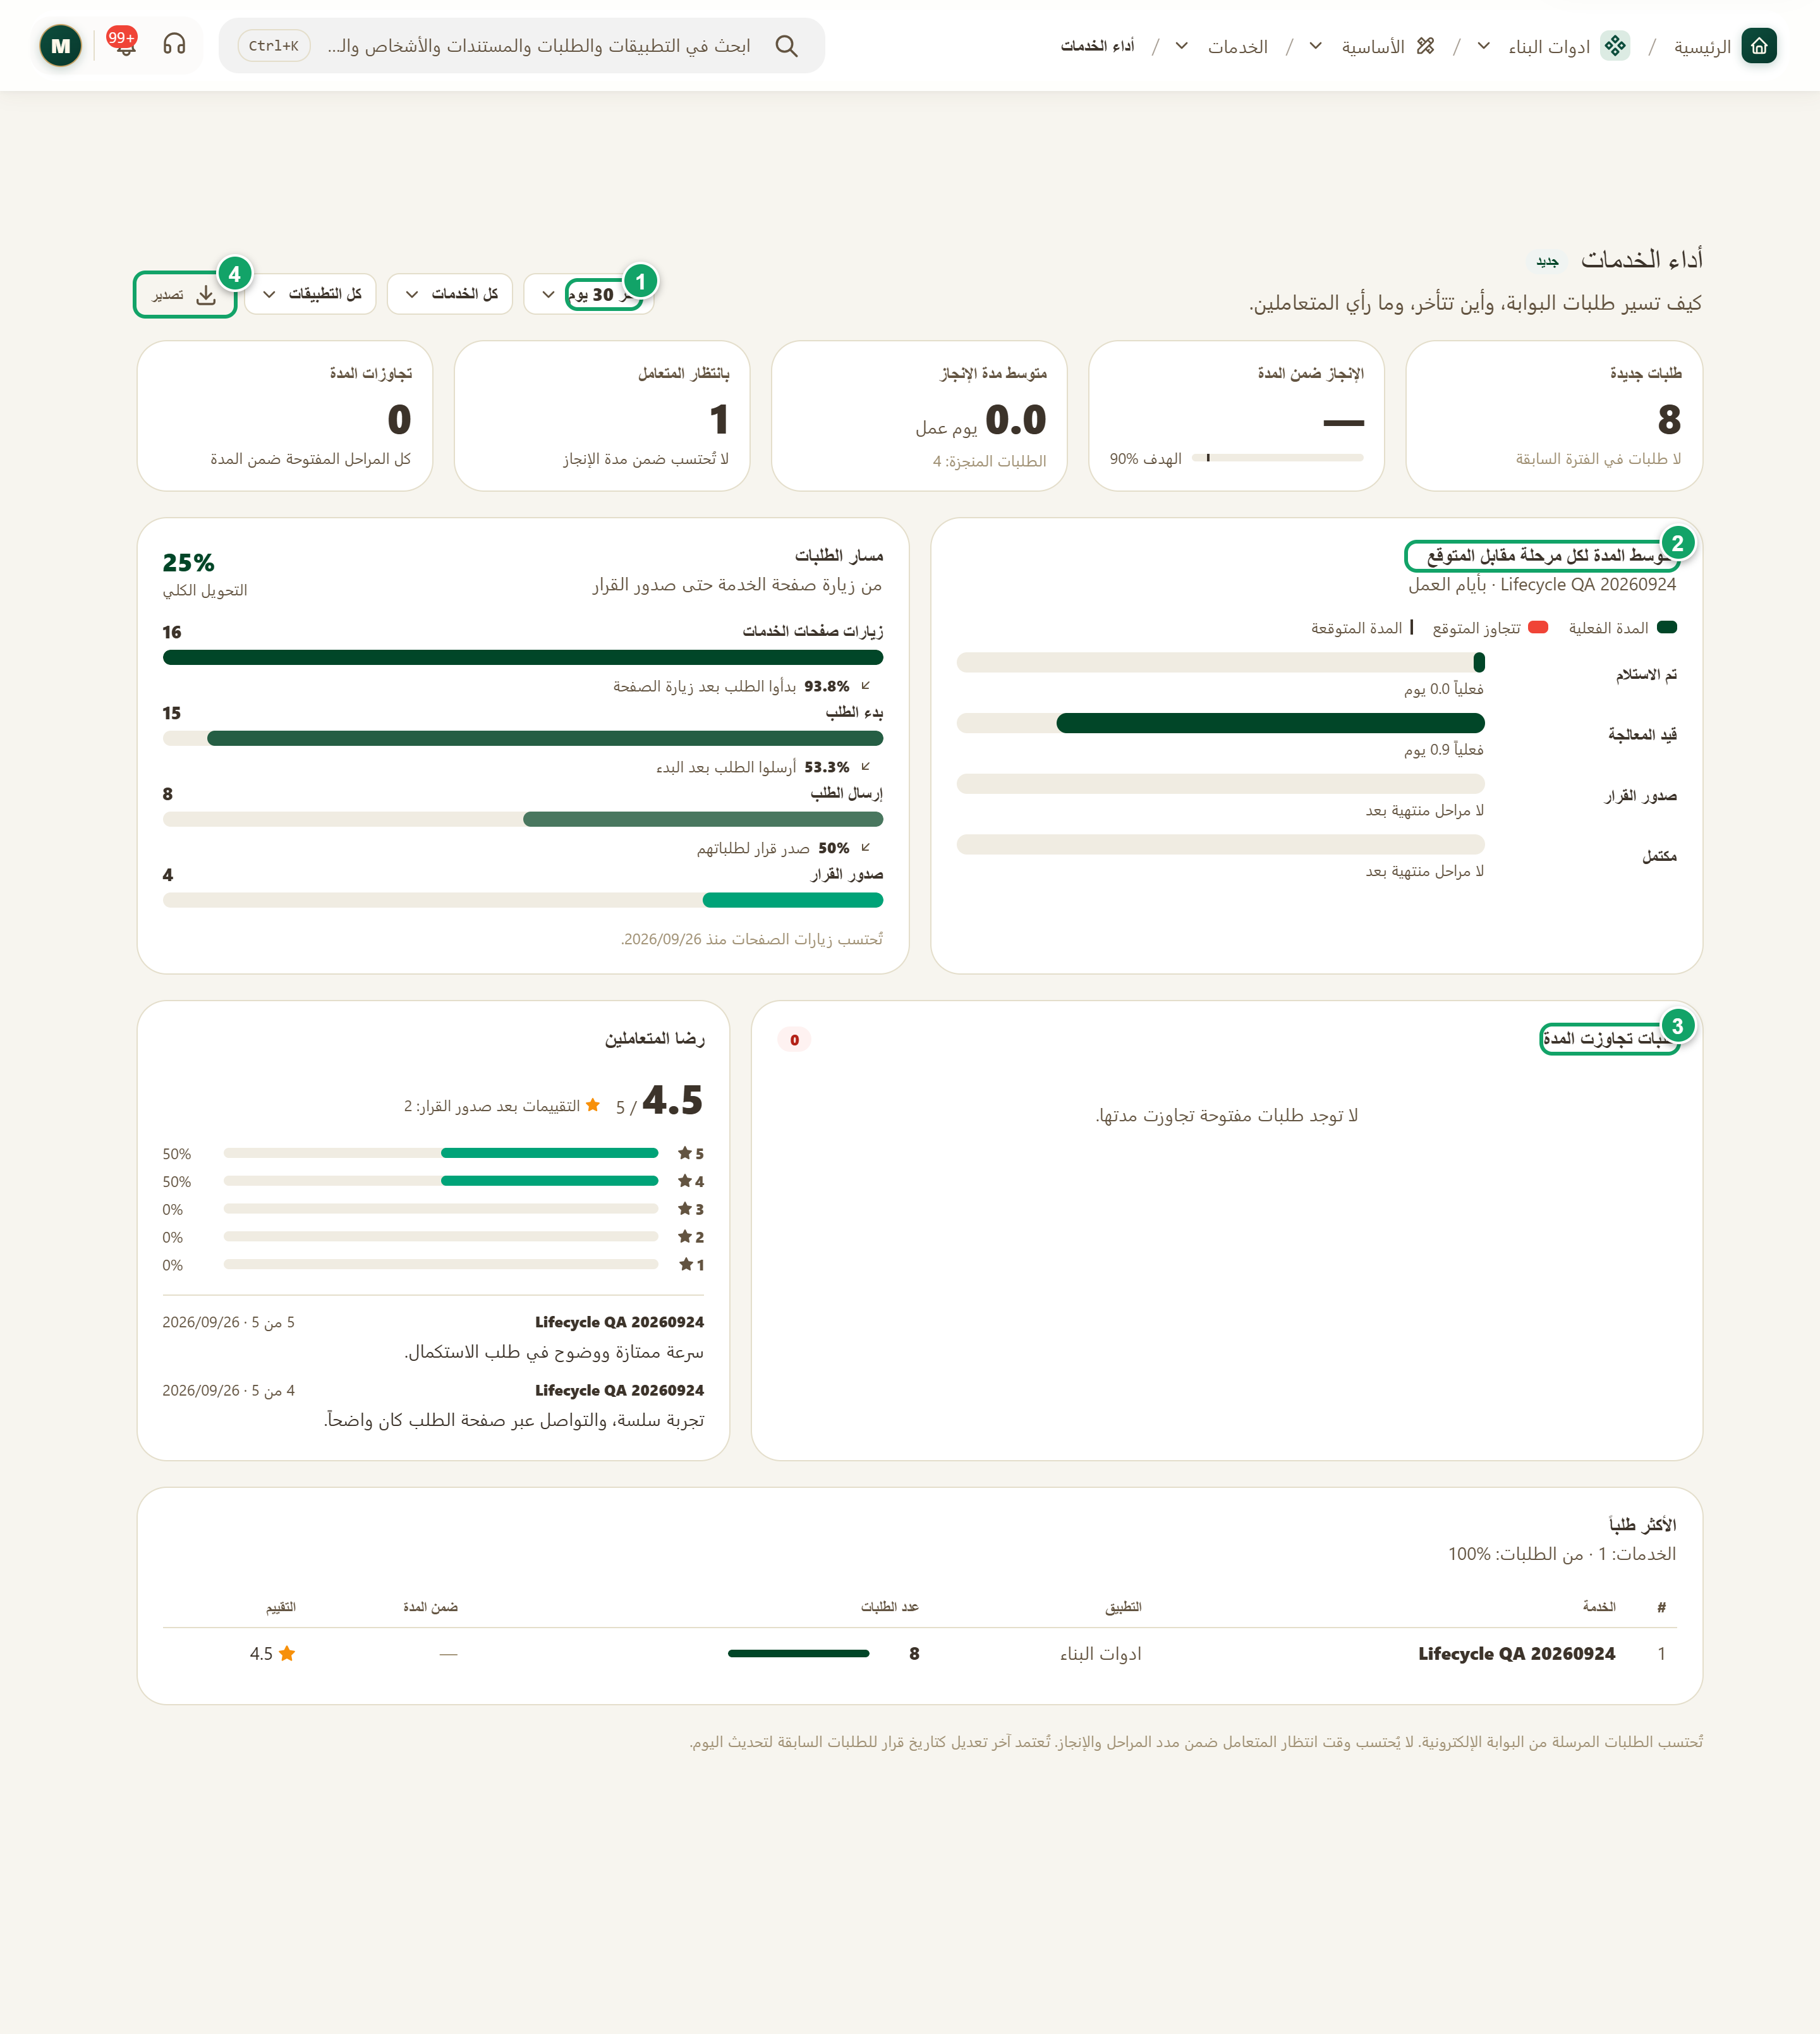
\includegraphics[width=0.95\linewidth,height=0.72\textheight,keepaspectratio]{figures/screens/ch06-services-performance-ar.png}
\caption{صفحة «أداء الخدمات»}
\label{fig:builder-services-performance-screen}
\shotnote{تعرض الصورة أداء خدمات مؤسسة الاختبار خلال آخر 30 يوماً، ولا يوجد فيها طلب تجاوز مدته، لذلك يظهر جدول التجاوزات فارغاً. وتبيّن أن الصفحة تنتقل من المؤشرات العامة إلى المراحل ثم إلى الطلبات الفردية. ① «آخر 30 يوم»: الفترة، وبجانبها تصفية الخدمة والتطبيق. ② «متوسط المدة لكل مرحلة مقابل المتوقع». ③ «طلبات تجاوزت المدة»: الطلبات المتأخرة مع زر «تصعيد». ④ «تصدير».}
\end{figure}

\begin{table}[H]
\centering
\caption{مؤشرات «أداء الخدمات»}
\label{tab:builder-services-performance-kpis}
\begin{tabularx}{\linewidth}{R{3.6cm} Y}
\rcHeaderRow
\thh{المؤشر} & \thh{ما يقيسه}\\
طلبات جديدة & عدد الطلبات في الفترة، مقارنة بالفترة السابقة.\\
الإنجاز ضمن المدة & نسبة المراحل التي انتهت في وقتها، مقابل هدف يظهر تحت المؤشر.\\
متوسط مدة الإنجاز & متوسط أيام العمل حتى صدور القرار، وعدد الطلبات المنجزة.\\
بانتظار المتعامل & الطلبات التي تنتظر إجراءً من مقدّمها، ولا تُحتسب ضمن مدة الإنجاز.\\
تجاوزات المدة & عدد الطلبات المفتوحة التي تجاوزت مدة مرحلتها، والمرحلة الأكثر تأخراً.\\
\end{tabularx}
\end{table}

\begin{table}[H]
\centering
\caption{بطاقات التحليل}
\label{tab:builder-services-performance-cards}
\begin{tabularx}{\linewidth}{R{3.6cm} Y}
\rcHeaderRow
\thh{البطاقة} & \thh{ما تعرضه}\\
متوسط المدة لكل مرحلة مقابل المتوقع & المدة الفعلية لكل مرحلة بأيام العمل مقارنة بالمدة المتوقعة المحددة في «المراحل والمدد» في النموذج، للخدمة المختارة أو الأكثر طلباً.\\
مسار الطلبات & من «زيارات صفحات الخدمات» إلى «بدء الطلب» ثم «إرسال الطلب» ثم «صدور القرار»، مع «التحويل الكلي».\\
طلبات تجاوزت المدة & «رقم الطلب» و«الخدمة» و«المرحلة» و«المسؤول» و«التجاوز»، مع زر «تصعيد».\\
رضا المتعاملين والأكثر طلباً & متوسط التقييمات بعد صدور القرار، وجدول الخدمات الأكثر طلباً مع نسبتها من الطلبات وتقييمها.\\
\end{tabularx}
\end{table}

\begin{figure}[H]
\centering
\begin{tikzpicture}[node distance=0.5cm]
\node[stepBox] (a) {\RL{الفترة والخدمة}};
\node[stepBox,below=of a] (b) {\RL{قراءة المؤشرات}};
\node[stepBox,below=of b] (c) {\RL{تحديد المرحلة المتأخرة}};
\node[stepBox,below=of c] (d) {\RL{تصعيد الطلبات المتأخرة}};
\node[stepBox,below=of d] (e) {\RL{التصدير للمراجعة}};
\draw[flowsTo] (a) -- (b);
\draw[flowsTo] (b) -- (c);
\draw[flowsTo] (c) -- (d);
\draw[flowsTo] (d) -- (e);
\end{tikzpicture}
\rclegend
\caption{مراجعة دورية لأداء الخدمات}
\label{fig:builder-services-performance-flow}
\shotnote{ينتقل المخطط من الصورة العامة إلى الطلب الواحد: المؤشرات تبيّن وجود تأخر، وبطاقة المراحل تحدد مكانه، وجدول التجاوزات يسمح بتصعيد كل طلب على حدة. ويأتي التصدير أخيراً ليحفظ نتيجة المراجعة في ملف.}
\end{figure}

\subsection{خطوات العمل والتحقق}
\begin{enumerate}
\item افتح «الخدمات» واضغط «أداء الخدمات».
\item اختر «الفترة»: 7 أو 30 أو 90 يوماً، ثم اختر الخدمة أو التطبيق إن أردت التضييق.
\item قارن المدة الفعلية بالمتوقعة في بطاقة المراحل، وحدد المرحلة التي تتجاوز المتوقع.
\item اضغط «تصعيد» بجانب كل طلب متأخر يحتاج إلى تدخل.
\item اضغط «تصدير» لتحفظ المؤشرات في ملف.
\end{enumerate}

\textbf{تحقق ومعالجة المشكلة:} بعد التصعيد يتحول الزر إلى «تم التصعيد» ولا يمكن الضغط عليه مرة أخرى. وإذا ظهر «لا توجد مراحل للمقارنة بعد.»، فحدد مراحل النموذج ومددها في «المراحل والمدد». وإذا ظهر «تعذّر تحميل أداء الخدمات.»، فأعد تحميل الصفحة.
